\documentclass[a4paper]{article}

\usepackage[T1]{fontenc}
\usepackage[utf8]{inputenc}
%\usepackage[ngerman]{babel}
\usepackage{times, graphicx, currvita, hyperref, longtable, float, caption, subcaption}
\usepackage{amsmath,amsfonts,amssymb, amsthm}%, dsfont, bbm, mathtools, stmaryrd}
\usepackage{fancyhdr}
\usepackage{color}
% \usepackage{pgf}
\usepackage{tikz}
\usetikzlibrary{patterns,decorations.markings,arrows,calc}
\usepackage[english]{babel}
\usepackage{paralist}
\usepackage{algorithm}
\usepackage{algpseudocode}%should also load algorithmicx
\usepackage{hyperref}

% \usepackage{wasysym}	% verschiedene Symbole, siehe http://rpi.edu/dept/arc/training/latex/LaTeX_symbols.pdf
\usepackage{marvosym}
\graphicspath{{Bilder/}}

\theoremstyle{definition}
\newtheorem{definition}{Definition}[section]
\newtheorem*{Def1}{Definition}
\newtheorem*{ex}{Example}

\newtheoremstyle{Tobi}{10pt}{}{}{}{\bf}{ }{\newline}{}
% die parameter sind: {name}{platz drueber}{platz drunter}{schriftart text}{einrueckung}{schriftart kopf}{Punktierung des Kopfes}{Platz zwischen kopf und text}

\theoremstyle{Tobi}
\newtheorem{prop}[definition]{Proposition}
\newtheorem*{Pro}{Proposition}
\newtheorem{theorem}[definition]{Theorem}
%\newtheorem*{le}{Lemma}
\newtheorem{lemma}[definition]{Lemma}
\newtheorem{cor}[definition]{Corollary}
\newtheorem*{conj}{Conjecture}
\newtheorem{obs}[definition]{Observation}

% \theoremstyle{remark}
% \newtheorem*{que}{Questions}
% \newtheorem*{claim}{Claim}
% \newtheorem*{note}{Note:}
% \newtheorem*{remark}{Remark}


\newcommand{\R}{\mathbb{R}}
\newcommand{\N}{\mathbb{N}}
% \newcommand{\F}{\mathbb{F}}
% \newcommand{\1}{\mathbbm{1}}
\newcommand{\Rn}{\mathbb{R}^n}
% \newcommand{\La}{\mathcal{L}}
% \newcommand{\D}{\mathcal{D}}
\newcommand{\Om}{\Omega}
\newcommand{\pa}{\partial}
\newcommand{\C}{\mathcal{C}}
\newcommand{\ph}{\varphi}

\setlength{\parindent}{0pt}

%define tikz picture elements setting global here as style for all tikz pictures
%this is to set arrow in middle of lines
\tikzset{->-/.style={decoration={markings, mark=at position .5 with {\arrow{#1}}},postaction={decorate}}}
\tikzset{vertex/.style={circle,fill=black!40}}
\tikzset{source/.style={circle,draw=green,fill= green!20}}
\tikzset{sink/.style={circle,draw=red,fill =red!20}}
\tikzset{every picture/.append style={scale=2.5}}%maybe better set locally?
\tikzset{edge/.style={semithick, solid}}%could also do dashed, dotted, double...
\tikzset{arc/.style={->-, semithick}}
\tikzset{fatarc/.style={very thick, ->-={latex}}}
\tikzset{edgeflow/.style={line width=3pt, #1!40}} %rounded corners funzt nicht?
\tikzset{arcflow/.style={->-, line width=3pt, #1!40}}
\tikzset{edgeflow/.default=blue}
\tikzset{arcflow/.default=blue}
\tikzset{->-/.default=stealth}
\tikzset{curvedarc/.style={arc, bend angle = 10, bend right}}
\tikzset{curvedarcflow/.style={arcflow, bend angle = 10, bend right}}
% \begin{figure}[h!]
% \centering
% \begin{tikzpicture}
% \node (s) at (0,0)[vertex, label=s]{};
% \draw[arcflow] (s)--(3)--(t);
% \end{tikzpicture}
% \caption{}
%  \label{bild:}
% \end{figure}

\begin{document}

\title{Entwurf MA - Bounds for Acyclic Network Flows}

\author{Tobias Buchwald}
% \maketitle

%\large{Bachelorarbeit bei Prof. Dr. Stefan Felsner}


% \begin{center} 
%TODO auf Masterarbeit anpassen
% \Huge{Domino Tilings auf dem Torus}\\ \vspace{12 cm}
% \Large{Bachelorarbeit\\ bei Prof. Dr. Stefan Felsner}\\ \vspace{1cm}
% \large{Vorgelegt von Tobias Buchwald}\\
% \large{am Fachbereich Mathematik der \\Technischen Universit�t Berlin}\\
% \vspace{2cm}
% \large{Berlin,  \today}
% 
% \end{center} 
% 
% 
% \textbf{Erkl\"arung}\\

Hiermit versichere ich an Eides statt, dass ich die vorliegende Masterarbeit selbst\"andig und eigenh\"andig sowie
ausschlie\ss lich unter Verwendung der aufgef\"uhrten Quellen und Hilfsmittel angefertigt habe. \\


Berlin, den \today
\newline

\rule[-0.2cm]{10cm}{0.5pt}

\textsl{Tobias Buchwald} 
% \newpage

\tableofcontents
\newpage
\section{Introduction} 
Today more and more real-world problems in the areas of simulation and optimization are solved by mathematical and 
computational methods. A growing number of these problems can be solved without problems, i.e. even huge instances give 
an optimal or near optimal solution within seconds. Still, there remain problems that even on modern computers are hard 
to solve. For these problems it is important to find ways to increase the efficiency of the algorithms. 

The topic of this thesis arises from the computation of flow in natural gas networks, which is currently developed 
in the FORNE Project in a cooperation of OGE with universities and research insitutes including ZIB.
%TODO genaueres zu FORNE? genaueres zum aufbau des Gasnetzes?
The flow of natural gas in a network is described by nonlinear equations and depends on many parameters, which makes 
the problem hard to solve. If we can find good upper and lower bounds for the flow on an arc during the preprocessing, 
we can hope to improve the behavior of the nonlinear solver by giving these tigther bounds. 

The flow is induced by pressure differences, so in reality there can't be cyclic flow (if we exclude compressor 
stations). Without the condition of acyclic flow, it is sufficient to run a standard min-cost-flow algorithm where the 
maximized arc $e$ gets weight $w_e = -1$ and all others are 0. However, the arising bounds are far from optimal. If arc 
$e$ is contained in any cycle we could decrease the cost by pushing more and more flow around this cycle until the arcs 
capacity is at its limits.

This master thesis will deal with the problem of finding a network flow with no directed cycles (acyclic flow), which at 
the same time maximizes the amount of flow on a specified arc $e$ of the network. We will discuss the complexity, an 
exact algorithm based on a mixed integer program with separation of inequalities that forbid cycles and also a heuristic 
approach that yields results much faster (but not optimal).%TODO am ende genauer schreiben was wirklich gemacht wurde

\subsection{The gas flow problem}
Although it is mainly the motivation, not really the topic of this thesis, we want to briefly introduce the gas 
transport problem. For more a detailed description we refer to LINK %TODO link auf ein entsprechendes ZIB-paper!!! 
\newpage
\section{Motivation}
Natural gas is one of the most common ressources of energy in germany and makes up more than 20 percent of energy 
consumption. Most of this gas is produced in ressource-rich countries like Russia or Norway and transported to Germany 
through special pipelines. 
%TODO wie sollte ich das projekt am besten referenzieren?
This thesis evolved from a joint research project of the Konrad Zuse Zentrum fuer Informationstechnik Berlin (ZIB) with 
Open Grid Europe (OGE) who operate the largest network of gas pipelines in germany. 
A general overview over the work done at ZIB on the gas network planning in this project is given in 
\cite{FuegenschuhGeisslerGollmeretal.2013}. The problem of finding settings for all active components of the network 
such that given (static) demands and supplies can be sent through the network with respect to all constraints is the 
\textit{nomination validation} problem. A description of the model used and work done at ZIB for the nomination 
validation problem can be found in \cite{PfetschFuegenschuhGeissleretal.2012}. 

The flow of gas through a pipeline network is determined by physical conditions such as pressure and temperature. 
Pressure can be increased in compressor stations and controlled by elements like valves. Pressure loss along a pipe is 
described by ordinary differential equations. 

The computation of such a physically exact flow is difficult due to numerical and algorithmical reasons. Good 
preprocessing routines can help a lot by reducing the domains and model sizes before the main computation is started.

Since the flow of gas in the network is always determined by pressure differences and flow is always going from higher 
pressure to lower pressure we know that flow in the network in general has to be acyclic. The only exception of this 
rule is a compressor station. Because active compressor stations increase
pressure it is possible that they cause cyclic flow. But of course in real gas networks a compressor station would 
normally be placed at a point where it has the highest impact. This is naturally at a place where it is unlikely to 
waste energy by sending flow on a cycle. The pressure would rather be controlled by resistors, valves and control valves 
in order to avoid cycing. So we will assume that the acyclic flow model is reasonable for the gas flow problem.\\

%erklärung warum wir engere Bounds brauchen können
The bounds are expected to be useful for two things in the solving process of the nomination validation problem 
described in \cite{PfetschFuegenschuhGeissleretal.2012}. If we have stronger bounds on the flow values in the network, 
it might improve the models that solve the actual nomination validation problem. 
%TODO detaillierter! Erst das Modell mit dem MIP beschreiben und dass es durch kleinere Intervalle die Zahl der vars 
%verringert
For the MILP approach described in \cite{PfetschFuegenschuhGeissleretal.2012} a linearization of the 
nonlinear model is computed. If the bounds are smaller or flow is even fixed to a specific value, the interval to be 
linearized is smaller. The smaller the interval, the less variables are needed. A small model might improve the running 
time / solvability of the model.

We also hope for improvements on the outer approximation with spatial branching approach. Here improved bounds could 
result in a stronger relaxation and thereby make solving the problem faster. \\
% TODO das MINLP beschreiben und wie sich im MINLP die Modellgroesse verkleinert?

So we set the goal to have good bounds and reduce problem size in order to reduce the overall running time of the 
nomination validation computations. To achieve this it is necessary to find the bounds quickly. This is why we also 
present relaxations/heuristics for the acyclic flowbound problem. The effects of the bounds on the MILP model reduction 
are shown in the last section of this thesis.



% We simplified the problem by assuming that there are no compressor stations or at least they do not cause cyclic flow. 
% At the same time we just ignore the physical properties of the gas. We do not compute or take care of any gas density, 
% pressure or possible pressure loss. Pressure is only used to justify the assumption of acyclicity. This abstraction is 
% justified by the fact that it is weaker than the original problem which also has to fulfill the flow conditions we use. 
% The bounds are only needed for preprocessing and to improve the model size in the end. 

\section{Related Work}
The diploma thesis of Thea Göllner \cite{DiplomarbeitTheaGoellner} describes preprocessing techniques for stationary gas 
network optimization models. This is the same model as the one we use here. In her thesis she also describes an 
algorithm for determining flow directions on the arcs of the network and determines cases in which we can fix the flow 
direction even on arcs contained in cycles of a certain kind. To achieve this she makes use of the acyclicity property 
of gas flow as well. 
Fixing a flow is basically saying that the lower flow bound in one direction is zero. Thus her work is a special case 
of the much more general approach on preprocessing with acyclic bounds we have in here. The fixing of flow directions 
that she proposes works on induced paths of the network and on cycles where flow can only be coming in from one side. 
She also shows the restrictions of this approach and says that for many cases it is necessary to take pressure or flow 
quantity into account in order to see if one can fix the direction variable. 

Here we aim at computing more general acyclic flow bounds. So we can not only fix the direction of flow in some special 
cases but also give upper bounds on possible flow and bounds in cases were it is not clear which direction flow has to 
take. It still yields flow directions in the cases described. But in practice a combination of our models with the 
flow direction fixing Göllner did could improve runtime and quality, because for big networks we can only use heuristic 
algorithms in practice.\\

Despite looking for other related work on acyclic network flows I could not manage to find publications dealing with this 
problem. This might be due to the fact that many applications just need some flow through a network without being 
interested in influencing its path, or that it is enough to make a flow acyclic by the shifting described here, or maybe
 I just searched the wrong places and did not discover it. 

\newpage
\subsection{Basic Notation and Definitions}% Als Referenz und Grundlage fuer die Definitionen nutze ich das Lehrbuch Combinatorial Optimization:Theory and 
%Algorithms von Bernhard Korte u Jens Vygen - definiere die wichtigsten Sachen aber erstmal auch selbst
\subsection{Graph Theory Basics}
Since there are many definitions in graph theory which may differ slightly, we want to introduce now the basic notation 
and definitions that we use throughout this thesis. The definitions in this chapter are mainly taken from the textbook 
about combinatorial optimization by Korte and Vygen \cite{KorteVygenCombOpt2007}.

\begin{definition}

An \textit{undirected graph} is a triple (V, E, $\Psi$), where $V$ and $E$ are finite sets and
$\Psi: E\to \{X \subseteq V: |X| = 2\}$. \\
A \textit{directed graph or digraph} is a triple $(V, E, \Psi)$,
where $V$ and $E$ are finite sets and $\Psi : E \to \{(v, w) \in V \times V : v \neq w\}$. 
In application to the gas problem we might call the graph modelling the gas infrastructure a \textit{network}. 
\end{definition}
 
The elements of $V$ are called \textit{vertices}, the elements of $E$ are called the \textit{edges}. $\Psi$ is the 
incidence function giving the relation between elements of $V$ and elements of $E$. 

In this thesis by a graph we normally mean the directed graph. If we talk about undirected graphs it will be stated 
explicitly. Edges of directed graphs will also be called \textit{arcs} to make clear that they are directed.\\

Two edges $e, e'$ with $\Psi(e) = \Psi ( e')$ are called parallel. Graphs without parallel
edges are called simple. For simple graphs we usually identify an edge $e$ with its
image $\psi(e)$ and write $G = (V(G), E(G))$ or $G=(V,E)$, where $E(G) \subseteq \{X \subseteq V(G) : |X| = 2\}$
or $E(G) \subseteq V(G) \times V(G)$. %We often use this simpler notation even in the presence
%of parallel edges, then the ``set'' $E (G)$ may contain several "identical'' elements. 
In this thesis all graphs are considered simple so we use this notation. 
%rausnehmen weil gar keine parallelen Kanten gebraucht werden
 
\begin{definition}
$|E(G)|=m$ denotes the number of edges and $|V(G)|=n$ denotes the number of vertices of a graph.
\end{definition}
\begin{definition}

We say that an edge $e = \{v, w\}$ or $e = (v, w)$ joins $v$ and $w$. In this case, $v$ and $w$ are \textit{adjacent}. 
$v$ is a \textit{neighbour} of $w$ (and vice versa). $v$ and $w$ are the \textit{endpoints} of $e$. If $v$ is an 
endpoint of an edge $e$, we say that $v$ is \textit{incident} with $e$. 
In the directed case we say that $e=( v, w)$ leaves $v$ and enters $w$,
$v$ is the \textit{tail} and $w$ is the \textit{head} of the arc $e$. 
Two edges which share at least one endpoint are 
called adjacent. 
\end{definition}

\begin{definition}
For a digraph $G$ the \textit{underlying undirected graph} is the undirected graph $G'$ on the same 
vertex set which contains an edge $\{v, w\}$
for each edge $(v, w)$ of $G$. We also say that $G$ is an orientation of $G'$.
\end{definition}
\begin{definition}
A \textit{subgraph} of a graph $G = (V(G), E(G))$ is a graph $H = (V(H), E(H))$
with $V(H) \subset V(G)$ and $E(H) \subset E(G)$. We also say that $G$ contains $H$. $H$ is an
induced subgraph of $G$ if it is a subgraph of $G$ and $E (H) = \{ \{x, y\} \textrm{ resp. } (x, y) \in
E(G) : x, y \in V(H)\}$. 
Here $H$ is the subgraph of $G$ induced by $V(H)$. 
\end{definition}
% A subgraph $H$ of $G$ is called spanning if $V(H) = V(G)$.

% If $v \in V(G)$, we write $G- v$ for the subgraph of $G$ induced by $V(G) \setminus {v}$.
\begin{definition}
For $e \in E(G)$, we define $G- e := (V(G), E(G) \setminus \{e\})$. Furthermore, the addition
of a new edge $e$ is abbreviated by $G + e := (V(G), E(G) \cup {e})$. 
% If $G$ and $H$ are two graphs, we denote by $G + H$ the graph with $V(G +H)= V(G) \cup V(H)$
% and $E(G +H)$ being the disjoint union of $E(G)$ and $E(H)$ (parallel edges may arise).
\end{definition}

% For a graph $G$ and $X, Y\subseteq V(G)$ we define $E(X, Y) := \{\{x, y\} \in E(G) : x \in
% X \setminus Y, y \in Y \setminus X\}$ resp. $E^+(X, Y) := \{(x, y) \in E(G) : x \in X\setminus Y, y \in Y \setminus 
% X\}$.
% For undirected graphs $G$ and $X \subseteq V(G)$ we define $\delta(X) := E(X, V(G) \setminus X)$. The
% set of neighbours of $X$ is defined by $ \Gamma(X) := \{v \in V(G) \setminus X : E(X, \{v\})  \neq \emptyset\}$.
% For digraphs $G$ and $X \subseteq V(G)$ we define $\delta^+(X) := E^+(x, V(G) \setminus X)$, $\delta^-(x) :=
% \delta^+(V(G) \setminus X)$ and $\delta(X) := \delta^+(x) \cup \delta^-(x)$. We use subscripts (e.g. $\delta_G(X)$) to
% specify the graph $G$ if necessary.
% 
% For singletons, i.e. one-element vertex sets $\{v\} (v \in V(G))$ we write $\delta(v) :=
% \delta(\{v\})$, $\Gamma(v) := \Gamma(\{v\}), \delta^+(v) := \delta^+(\{v\})$ and $\delta^-(v) := \delta^-(\{v\})$. 
% The 
% degree of a vertex $v$ is $|\delta(v)|$, the number of edges incident to $v$. In the directed case, the
% in-degree is $|\delta^-(v)|$, the out-degree is $|\delta^+(v)|$, and the degree is $|\delta^+(v)|+ |\delta^-(v)|$.
% A vertex $v$ with zero degree is called isolated. A graph where all vertices have
% degree $k$ is called $k$-regular.
\begin{definition}
For undirected graphs $G$ and a set of vertices $X \subseteq V(G)$ we define the cut induced by $X$
$$\delta(X) := \{\{x, y\} \in E(G) : x \in X , y \in V(G) \setminus X\}$$
%The set of neighbours of $X$ is defined by $ \Gamma(X) := \{v \in V(G) \setminus X : E(X, \{v\})  \neq \emptyset\}$.
For digraphs $G$ and $X \subseteq V(G)$ we define 
$$\delta^+(X) := \{(x, y) \in E(G) : x \in X , y \in V(G) \setminus X\}$$ and
$$\delta^-(X) := \{(y, x) \in E(G) : x \in X , y \in V(G) \setminus X\}$$
% and $\delta(X) := \delta^+(x) \cup \delta^-(x)$. 
 
For one-element vertex sets $\{v\}$ (with $v \in V(G))$ we write $\delta(v) :=\delta(\{v\})$ for the set of incident 
edges of $v$, and in the directed case 
$ \delta^+(v) := \delta^+(\{v\})$ for the outgoing arcs and $\delta^-(v) := \delta^-(\{v\})$ for the set of ingoing 
arcs of $v$
\end{definition}
We use subscripts (e.g. $\delta_G(X)$) to specify the graph $G$ if necessary.
\begin{definition}
The \textit{degree} of a vertex $v$ is $|\delta(v)|$, the number of edges incident to $v$. In the directed 
case, the in-degree is $|\delta^-(v)|$, the out-degree is $|\delta^+(v)|$, and the degree is 
$|\delta^+(v)|+ |\delta^-(v)|$.
\end{definition}
A vertex $v$ with zero degree is called isolated. A graph where all vertices have degree $k$ is called $k$-regular.

\begin{definition}
An \textit{edge progression} $W$ in $G$ is a sequence $v_1, e_1, v_2, \dots , v_k, e_k, v_{k+1}$ such that $k 
\ge 0$, and $e_i = (v_i, v_{i+ 1}) \in E(G)$ resp. $e_i = \{v_i, v_{i+1}\}\in E(G)$ for $i = 1, \dots , k$. If in
addition $e_i \ne e_j \,\forall\, 1 \le i < j \le k$, $W$ is called a \textit{walk} in $G$. $W$ is \textit{closed} if
$v_1 = v_{k+1}$. 

A \textit{path} is a graph $P = (\{v_1, ... , v_{k+1}\}, \{e_1, ... , e_k\})$ such that $v_i \ne v_j$ for
$1 \le i < j \le k + 1$ and the sequence $v_1 , e_1 , v_2, \dots , v_k, e_k, v_{k+1}$ is a walk. $P$ is
called a path from $v_1$ to $v_{k+1}$ or a $v_1 - v_{k+1}$-path. $v_1$ and $v_{k+1}$ are the endpoints
of $P$.
% By $P_{[x,y]}$ with $x, y \in V(P)$ we mean the (unique) subgraph of $P$ which is an $x-y$-path. 
 
\end{definition}
Evidently, there is an edge progression from a vertex $v$ to another vertex $w$ if and only if there is a $v-w$-path.
\begin{definition}

A \textit{cycle} is a graph $(\{v_1, \dots , v_k\}, \{e_1, \dots, e_k\})$ such that the sequence $v_1, e_1, v_2, 
\dots , v_k,e_k,v_1$ is a (closed) walk and $v_i \ne v_j$ for $1 \le i < j\le k$.
 
\end{definition}
An easy induction argument shows that the edge set of a closed walk can be partitioned into edge sets of cycles.

%eingefuegt: definition kreisbasis
\begin{definition}
 For cycles $C_1$, $C_2$ in a graph we define a cycle addition operation or sum of cycles as symmetric difference 
 $C_1+C_2=(C_1\cup C_2)\setminus (C_1\cap C_2)$. 
 
 With this operation we can define a \textit{cycle base} as a minimal 
set of cycles $\mathbb{B}=\{C_1,C_2,\dots, C_l\}$ such that we can represent every possible cycle in the graph as sum 
$\sum_{i=1}^k C_i\,|\C_i\in\mathbb{B}$ of cycles in the cycle base.
\end{definition}

 
\begin{definition}
The length of a path or cycle is the number of its edges. If it is a subgraph of $G$, we speak of a path or cycle in 
$G$. 
\end{definition}

\begin{definition}
A spanning path (i.e. a path containing all vertices) in $G$ is called a \textit{Hamiltonian path} while a spanning 
cycle in $G$ is called a \textit{Hamiltonian cycle}. A graph containing a Hamiltonian cycle is a \textit{Hamiltonian 
graph}.
\end{definition}

\begin{definition}
 A \textit{ connected component } of a graph $G$ is a subgraph $G'\subseteq G$ such that there is a path in $G'$ from 
 every node $v\in G'$ to every other node $u\in G'$. We call a graph $G$ that forms a connected component on its own 
 \textit{connected}. 
\end{definition}


\begin{definition}
For two vertices $v$ and $w$ we write $dist(v, w)$ or $dist_G (v, w)$ for the length of
a shortest $v-w$-path (the \textit{distance} from $v$ to $w$) in $G$. If there is no $v-w$-path at all,
i.e. $w$ is not reachable from $v$, we set $dist(v, w) := \inf$. In the undirected case,
$dist(v, w) = dist(w, v)$ for all $v, w \in V(G)$.
\end{definition}

\begin{definition}

We shall often have a cost function $c : E(G) \to \R$. Then for $F \subseteq E(G)$ we
write $c(F) := \sum_{e\in F} c(e)$ (and $c(\emptyset) = 0$). This extends $c$ to a modular function
$c : 2^{E(G)}\to \R$. Moreover, $dist_{(G,c)}(v, w)$ denotes the minimum $c(E(P))$ over all
$v-w$-paths $P$ in $G$.
 
\end{definition}

\subsection{Combinatorial Optimization}
%TODO
Optimization of mathematical problems including to make certain discrete decisions is an important field of application 
for modern mathematics. The acyclic flow problem we describe in this thesis is a typical example of a combinatorial, 
graph theoretical optimization problem. Here we define such problems in general as well as the basics of integer 
programming which is a standard approach to solve such problems. 

The definitions are taken from the scriptum of the course ADM I by Martin Gr\"otschel held in 2012/2013, see 
\cite{groetschelSkript}. %TODO referenz

\begin{definition}
 Given a finite set $\mathcal{I}$ and a function $f:\mathcal{I}\to\R$. The problem of finding the element 
$i\in\mathcal{I}$ such that $f(i)$ is maximum or minimum is a general \textit{combinatorial optimization problem}.
\end{definition}
Of course it is hard to solve such a problem without having any structure on it. But the problems we have to deal with 
normally have  a good structure on them: The set $\mathcal{I}$ is defined implicitly by some conditions on its elements 
and the function $f$ is defined by formulas.

\begin{definition}
 Given some finite set $E$ , a set $\mathcal{I}\subset \mathcal{P}(E)$ of feasible solutions and a function 
 $c:E\to \R$. Define for a set $S \in \mathcal{P}(E)$ the total costs $c':\mathcal{P}(E)\to \R$, 
 $c'(S)=\sum_{s\in S}c(s)$. 
 
 The problem of finding an element $i_m\in\mathcal{I}$ with $c'(i_m)\ge c'(i)\forall 
 i\in\mathcal{I} $ (or $c'(i_m)\le c'(i)\forall i\in\mathcal{I} $) we call a \textit{combinatorial maximization 
(minimization)  problem} with linear objective function.
\end{definition}

Often we can model such combinatorial optimization problems as linear, mixed-integer, quadratic or constraint program 
depending on the definition of the feasible set $\mathcal{I}$. 

As we will make use of such programs we want to define the basics here. We use the framework SCIP ("Solving Constraint 
Integer Programs") for solving our problem. For details of the solver setup we refer to the PhD Thesis of Tobias 
Achterberg \cite{Achterberg2007} where he describes the main design of his Constraint Integer Programming solver SCIP. 
The following definitions also follow the work of Achterberg \cite{Achterberg2007}.

\begin{definition}
 A \textit{constraint program} is a triple $(\mathcal{C},\mathcal{D},f)$ and consists of solving
 $$f^*=\min\{f(x)|x\in \mathcal{D}, \mathcal{C}(x)\}$$ 
 with $\mathcal{D}=\mathcal{D}_1\times \dots\times \mathcal{D}_n$ the domain set, $f:\mathcal{D}\to\R$ the objective 
function and $\mathcal{C}=\{\mathcal{C}_1\dots \mathcal{C}_m\}$ the constraint set.
\end{definition}

As a special case of constraint programs that can be handled by computers and can be used to model many different 
combinatorial optimization problems we have mixed integer programs (or shortly referred to as MIP). Here the 
constraints and the objective function can be given as linear inequalities and in addition the domains of some 
variables can be restricted to integer values. Often variable domains are even more specifically restricted to 
$\{0,1\}$. The regarding variables are called binary (decision) variables.

\begin{definition}
 A \textit{mixed integer program} or \textit{MIP} is a constraint program with the following representation:\\
 Given a matrix $A\in\R^{m\times n}$, vectors $c\in\R^n$ and $b\in \R^m$ and a set $\mathcal{I}\subseteq \{1\dots n\}$ 
 we have to solve
 $$c^*=\min\{c^T x|Ax\le b, x\in\R^n, x_j\in\mathbb{Z}\textrm{ for all }j\in\mathcal{I} \}$$
 We call all the vectors x in the set
 $$X_\textit{MIP}=\{x\in\R^n|A x\le b, x\in\R^n, x_j\in\mathbb{Z}\textrm{ for all }j\in\mathcal{I} \}$$
 i.e. vectors fulfilling the constraints of the problem, the \textit{feasible solutions} of the MIP. A vector $x'\in 
 X_\textit{MIP}$ with $c^*=c^Tx'$ is called an \textit{optimal solution} of the MIP.
\end{definition}

There are important special cases of mixed integer programs: The set $\mathcal{I}$ of integer variables could be empty 
so we really just optimize over a polyhedron. This kind of MIP with $\mathcal{I}=\emptyset$ is called a \textit{linear 
program} or \textit{LP}. 

It can also happen that every variable is integer, i.e. $\mathcal{I}=\{1,\dots, n\}$. We call this MIP an 
\textit{integer program} or \textit{IP} in this case.

Solving linear programs can be done in polynomial time. Algorithms to achieve this were described by 
Khachiyan\cite{KHACHIYAN198053} and Karmarkar \cite{Karmarkar:1984:NPA:800057.808695}. Integer programs and by this 
also their generalization mixed integer programs can be (and mainly are) used for modeling $\mathcal{NP}$ hard 
problems. So unless $\mathcal{P}=\mathcal{NP}$ there is no polynomial algorithm to solve them.

Thus the LP relaxation of a MIP is a very important problem.
\begin{definition}
 The \textit{LP-relaxation} of a mixed integer program 
 $$\min\{c^T x|Ax\le b, x\in\R^n, x_j\in\mathbb{Z}\textrm{ for all }j\in\mathcal{I} \}$$
 is the MIP without any integrality constraints:
 $$\min\{c^T x|Ax\le b, x\in\R^n \}$$
\end{definition}

It can be solved efficiently since it is a linear program. The solution of the LP relaxation of a problem gives a
bound on the solution of the mixed integer problem. It is used to get a starting 
point for a branching process or for cutting planes, heuristics etc. that might yield an optimal or nearly optimal 
solution. 

\newpage
\subsection{The Acyclic Flowbound Problem}We already described the gas flow problem, where the motivation for this thesis came from. Here we want to define the 
problem as a general combinatorial flow problem with specific contraints. We will also give the formulation as a Mixed 
Integer Program (MIP) and as well some natural relaxations, which might be easier to solve.

We will represent our originally undirected graph by a directed graph where flow is allowed to go over edges backward 
and forward as well. This allows us to specify directions forward and backward on every edge in a consistant way. 


\begin{definition}
 Let $G=(V,A)$ be a directed Graph and $e \in A$ a specific arc of $G$. For every vertex $v\in V$ let there be a 
prescribed range for the amount of flow demand $[d_l(v), d_u(v)]\subset \R \setminus \{0\}$. Vertices with demand 
values greater than 0 are sinks, vertices with negative demand value are sources. In a feasible solution flow 
demands are assumed to be balanced on their (absolute) higher bound values 
$$\sum_{v \in V\textrm{ sink}}d_u(v)-\sum_{v \in V\textrm{ source}}d_l(v)=0$$ 
%TODO am ende kontrollieren, dass demands (was positiv, was negativ) konsistent verwendet wurde!

Let there be a capacity function 
$$c:A\to \mathcal{P}(\R), \, c(a)=[c_l(a), c_u(a)],\, c_l(a)\le 0 \le c_u(a) \, \forall a\in A$$
and a flow  $f: A\to \R $ with $$c_l(a)\le f(a)\le 
c_u(a)\, \forall a\in A$$ and $$\sum_{a\in\delta^-(v)}f(a)-\sum_{a\in\delta^+(v)}f(a)-d(v) = 0 \, \forall v\in V$$
We call this a \textit{feasible network flow on G}, i.e. a flow with balances of 0 and respected capacity bounds.
We also call $$\sum_{a\in \delta^-(v)}f(a)-\sum_{a\in\delta^+(v)}f(a)-d(v)$$ the flow balance, which might be nonzero 
in incomplete flows during a solving algorithm.\\
\end{definition}

The standard definition of Flow Problems has fixed demand values $d(v)=const$ instead of an interval. These two 
definitions are equivalent in the way that you can transform them into each other easily in polynomial time. Obviously 
we can see fixed demands $d(v)$ as intervals with $d_l(v)=d_u(v)=d(v)$ consisting of only one point $[d(v), d(v)]$. The 
other way around we use a construction that adds only one node and $|\{v\in V| d_u(v)<0\}|+|\{v\in V| d_l(v)>0\}|$ arcs 
to the network.
\begin{prop}
 There is a (linear time) transformation from the flow problem with demand intervals on the vertices to the standard 
flow problem with fixed demands. 
\end{prop}
\begin{proof}
 Given a graph $G=(V,A)$ with demand intervals at the entries and exits, we construct a graph $G'=(V',A')$ as follows:
 $$V' := V\cup \{z\} \textrm{, and } A' := A\cup \{ (v,z)| d_u(v)<0 \}\cup\{ (z,v)|d_l(v)>0\}$$ On $G'$ we then have 
to redefine the arc capacity and node demands: 
$$c':A\to \mathcal{P}(\R)  \,, c'(a)= c'(u,v) = \begin{cases} \{x|x\in [0,d_u(u)-d_l(u)]\} &\textrm{if }v=z\\ 
\{x|x\in [0,d_u(v)-d_l(v)]\}&\textrm{if }u=z\\ \{x|x\in[c_l(a), c_u(a)]\} &\textrm{else } \end{cases}
$$ 
The node demands now are 
$$ d'(v)=\begin{cases} d_l(v) & \textrm{if v is source, i.e. }d_u(v)<0\\
         d_u(v) &\textrm{if v is sink, i.e. }d_u(v)>0
        \end{cases}
$$
If we compute a solution of the flow problem on $G'$ and restrict the flow to the arcs of $G$, we get the solution of 
the problem on $G$ that respects the demand intervals:\\ 
We call the demands in the solution restricted to arcs of $G$ $d^s$ and have $ d^s(u)=d'(u)+f'((u,z))$. The flow balance 
constraints in normal nodes 
(nodes with demand 0) do not change at all, since the only new node $z$ is not in their neighborhood. All vertices that 
are sources or sinks (per definition thy cannot be both at the same time) have $z$ as neighbor. The flow balance on a 
source $u$ before and after restriction to $G$ differs only by the flow on the artificial arc $(u,z)$. This flow 
$f'((u,z))$ is in the capacity range $[0,d_u(u)-d_l(u)]$. Hence for sources $u$ ($d'(u)<0$) with 
$d^s(u)=d'(u)+f'((u,z))$ we can conclude for the demands $d^s(u)$ of the solution restricted to $G$ 
$$d_l(u)\le d^s(u)=d'(u)+f'((u,z))=d_l(u)+\underbrace{f'((u,z))}_{0\le f'((u,z))\le d_u(u)-d_l(u)} \le d_u(u)$$
and as well for sinks ($d'(v)>0$)
$$d_l(v)\le d_u(v)-\underbrace{f'((z,v))}_{0\le f'((z,v))\le d_u(v)-d_l(v)}=d'(v)-f'((z,v))=d^s(v) \le d_u(v)$$
\end{proof}



 %cycle was already defined in the Definitions chapter
\begin{definition}
A \textit{cyclic flow} within such a feasible network flow $f$ is a flow $f':C\to \R$ where $C\subseteq A$ is a cycle, 
$$\sum_{a\in \delta^+(v)\cap C}f(a)-\sum_{a\in\delta^-(v)\cap C}f(a) = 0 \, \forall v\in C$$ for all arcs the flow 
directions in $f'$ and $f$ are the same, i.e. $f(a)\ge 0\Rightarrow f'(a)\ge 0,\, f(a)\le 0 \Rightarrow f'(a)\le 0$ and 
there is really a nonzero flow, i.e. $f'(a) \ne 0 \,\forall a\in C$. 

If there is any cyclic flow $f'$ in a network flow $f$ we say that $f$ contains a flow cycle. If there is no cyclic 
flow, we say $f$ is \textit{acyclic} or an \textit{acyclic flow} on $G$.\\

The conditions imply, that a cyclic flow is one that has no sources or sinks and the same value of flow on each arc.

The \textit{size of a cyclic flow} is the absolute amount of of flow contributing to the cycle. This means it is the 
maximum value $|f'(a)|$ a cyclic flow $f'$ can reach. 
%flow $ f: C\to \R ,\, C\subseteq A \textrm{ a cycle, }\,c_l(a)\le 
%f(a)\le c_u(a)\, \forall a\in C$ with the property that 
\end{definition}
%TODO Kreisflussmenge, Kreisflusskapazität, Augmentierung


\begin{definition}
  Given a graph $G=(V,A)$ like above, with $e \in A$ a specific arc of $G$. 
  
  We call the problem of finding an acyclic flow $f:A\to \R$ with $f(e)\ge f'(e)\,\forall f':A\to \R \textrm{ s.t.} f' 
\textrm{ is an acyclic flow on }G$ the \textit{ Edge-Maximizing Acyclic Flow Problem}.
\end{definition}

\begin{prop}
  The maximal flow value on the maximized arc $e$ in the Edge-Maximizing Acyclic Flow Problem is the same as the 
  maximal flow value if only cycles containing $e$ are forbidden. 
\end{prop}
\begin{proof}

 Let $F_{acyc}$ be the set of flows that are really acyclic and $F_{cyc}^e$ the flows that can have cyclic flow on 
 cycles not containing $e$. Since $F_{acyc}\subseteq F_{cyc}^e $ (i.e. the partially cyclic flow problem is a 
 relaxation of the acyclic problem) we always have $f_{cyc}(e)\ge f_{acyc}(e)$ for all $f_{cyc}\in F_{cyc}^e, 
f_{acyc}\in F_{acyc}(e)$ that are maximizing flow on $e$. We have to show that also $f_{cyc}(e)\le f_{acyc}(e))$.
% Every two flows differ only by a sequence of cyclic flow augmentations in the network. Thus if not $f_{cyc}(e)\le 
% f_{acyc}(e)$ we can choose a pair $f,f'$ such that $f$ is completely acyclic and $f'$ is not, $f'(e)>f(e)$ and that 
% $f'$ differs from $f$ by just one cyclic shift of flow (take the first flow of the sequence where $f'(e)>f(e)$).

%%%%%%%%%%%%%%%%%%%%%%%%%%%%%%%%%%%%%%%%%%%%%%%
%observation: it is always easier to look at a cycle and ask how much flow can you send from one node to another. this 
%not changing, never, by a cyclic flow. but a cyclic flow could affect other cycles. But since we do not have any 
% lower bounds higher than 0 we can always shift a cyclic flow until it is acyclic!!!
%%%%%%%%%%%%%%%%%%%%%%%%%%%%%%%%%%%%%%%%%%%%%%%
% In $f_{cyc}$ there are no cyclic flows on the maximized arc $e$. Take a solution of $f_{cyc}$ with cyclic flow on a 
% simple cycle $C\in A(G)$. There is no minimum flow higher than 0. Thus it is always possible to shift the cyclic flow 
% backwards on the cycle by the minimum amount of flow on this cycle. This is a cyclic flow, so on every arc $a\in C$ the 
% flow value $f(a)$ is decreased by this. However, there is no arc where flow directions are changed. We can do this 
% operation as long as there is cyclic flow without changing flow value on $e$ or creating new flow cycles. In the 
% end we get an acyclic flow with the same flow value.
We show how we can produce a completely acyclic flow $f'\in F_{acyc}$ from any given flow $f_{cyc}\in F_{cyc}^e$. 

This flow will have the same flow value on $e$: $f'(e)=f_{cyc}(e)$ , so for each flow $f\in F_{cyc}^e$ there is an 
acyclic flow with at least the same flow value on $e$.\\
Take a given flow $f\in F_{cyc}^e\setminus F_{acyc}$. Consider a cycle $C$ where $f$ has cyclic flow. On $C$ all flow 
is going in the same direction. Choose the minimum flow value $\alpha(C)=\min(f(a)|a\in C)$ on an edge of $C$ and 
decrease flow on every edge of $C$ by $\alpha$. On no arc the direction of flow was reversed, so no new cyclic flows
are created by this. But on one arc at least there is no flow at all, so on $C$ we have no cyclic flow anymore. The 
resulting flow is still a valid flow: On each node ingoing and outgoing flow is decreased by the same value $\alpha$ so 
flow balances still hold. The capacity constraints are still fulfilled because we know that no minimum flow bound is 
higher than 0 in our problem. The flow on the special arc $e$ is unchanged, since $e$ must not be contained in any 
cyclic flow.

We can continue this until there is no cyclic flow left and we transformed our flow into a flow $f'\in F_{acyc}$ with 
the same flow value on $e$ as before. The algorithm terminates after less than $|A(G)|$ repetitions because every arc 
can be set to zero only once.\\
$\Rightarrow $ We conclude that $\max(f(e)|f\in F_{cyc}^e)\le \max(f'(e)|f'\in F_{acyc})$ and together with 
$F_{acyc}\subseteq F_{cyc}^e $ this yields
$$\Rightarrow \max(f(e)|f\in F_{cyc}^e)= \max(f'(e)|f'\in F_{acyc}) $$
\end{proof}


Now that we defined our problem, we can investigate it deeper. The acyclic Flowbound Problem is obviously closely 
related to other flow problems, 
though the special constraints we built make it more complicated. One way to deal with this is to look at related 
problems, which could give bounds on our problem or even the same solution in special cases.

\subsubsection{Relation To Other Flow Problems/Relaxations}
\label{sect:mincostflow}
If we look for related problems, it is natural to just drop the constraints of our problem. In this case we could for 
example easily forget the contraint that flows have to be acyclic. If we do this, our problem becomes a special 
instance of a Min-Cost-Flow where we allow edge weights to be negative:

\begin{definition}\label{def:mincostflow}
 The \textit{Minimum Cost Flow Problem} is the problem to determine a feasible network flow with the least possible 
cost $c_f$. The cost function $c:A\to \R$ (or often $c:A\to \R_{\ge 0}$) is defined on every arc, the cost of the flow 
is $c_f = \sum_{a\in A}|f(a)|\cdot c(a)$. So for a given network and cost function we look for a flow $f$ s.t. $c_f\le 
c_{f'}\forall f':A\to \R$.
\end{definition}

This problem is normally defined with nonnegative cost functions, like in \cite{EdmondsKarp1972} where 
Jack Edmonds and Richard Karp present their well known $O(V\cdot E^2)$ flow algorithm. At least cycles of negative 
weight should be excluded, since they lead to problems in the algorithm's subroutines like shortest path. Nevertheless 
there are algorithms that can handle negative cycles without a problem - but they will of course give a solution 
where as much flow as possible is just flowing around these negative cycles. 
%, and make the problem hard. We will proof the hardness of this problem later.TODO auch ohne kreisfreiheit?

In our application we want to find upper and lower bounds on the possible flow over each arc. For this we set the 
weight on the arc $e$ where we want to maximize flow to -1 and compute a Minimum Cost Flow in the graph. If $e$ is 
contained in a cycle of $G$ whose arcs all have a very high upper capacity bound, $e$ will get a very high bound as 
well. The reason is that any cyclic flow over $e$ can reduce the cost of the flow. Hence as much cyclic flow as 
possible will be used to obtain a Minimum Cost Flow. 

So in most cases the bound computed with a Min-Cost Flow algorithm is not sharp. Still it gives an upper bound for the 
possible flow. Hence one could ask how good this bound will be, and whether we can use it as an approximation. It turns 
out that the gap between the amount of flow on an arc $e$ in an acyclic flow and in a possibly cyclic flow can be 
arbitrarily large:

\begin{prop}
 The gap between the maximum flow values $f(a)$ on an arc $a\in A$ in a normal and in an acyclic flow problem is 
unbounded. 
\end{prop}
\begin{proof}
 In order to show this we look at the two examples:
 \begin{figure}[h!]
  \centering
  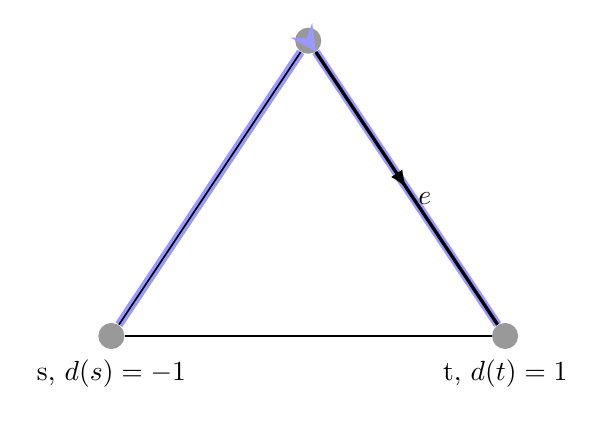
\begin{tikzpicture}
  \node (s) at (0,0)[vertex, label=below:{s, $d(s)=-1$}]{};
%   \node (stext) at (-0.1, -0.2){s, $d(s)=1$};
    \node (t) at (2,0)[vertex, label=below:{t, $d(t)=1$}]{};
%   \node (ttext) at (2.1, -0.2);
  \node (3) at (1,1.5)[vertex]{};
%   \node(etext) at (1.7,0.9){e};

  % \draw [edgeflow] (s)--(3);
  \draw[arcflow] (s)--(3)--(t);
  \draw [edge](s) -- (3);
  \draw [edge](s) -- (t);
  \draw[fatarc] (3) -- (t)node [pos=0.6, above] {$e$};;
  \end{tikzpicture}
 \caption{A simple network with acyclic flow}
 \label{bild:acyclicTriangle}
 \end{figure}
 
 \begin{figure}[h!]
  \centering
  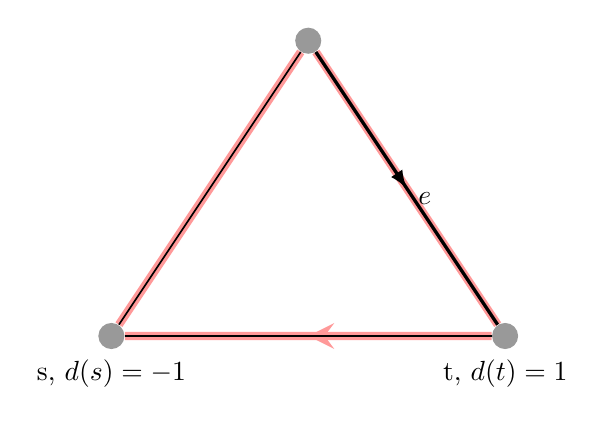
\begin{tikzpicture}
  \node (t) at (2,0)[vertex, label=below:{t, $d(t)=1$}]{};
  \node (s) at (0,0)[vertex, label=below:{s, $d(s)=-1$}]{};
  \node (3) at (1,1.5)[vertex]{};

  \draw[arcflow=red] (s)--(3)--(t)--(s)--(3)--(t);
  \draw [edge](s) -- (3);
  \draw [edge](s) -- (t);
  \draw[fatarc] (3) -- (t)node [pos=0.6, above] {$e$};
  \end{tikzpicture}
 \caption{The same simple network with cycling flow that can pass $e$ several times}
 \label{bild:cyclicTriangle}
 \end{figure}
In figure \ref{bild:acyclicTriangle} we see that the flow on the maximized arc $e$ in the acyclic case has to be 1. 
If we allow cyclic flow as in figure \ref{bild:cyclicTriangle} it could be any number - it is the minimum we choose as 
capacity for an arc in the network. Hence the relative gap is
$$ \frac{f_{cyc}(e)}{f_{acyclic}(e)}=\frac{\textrm{min capacity on the cycle}}{1}$$ which is unbounded.

  
\begin{figure}[h!]
\centering
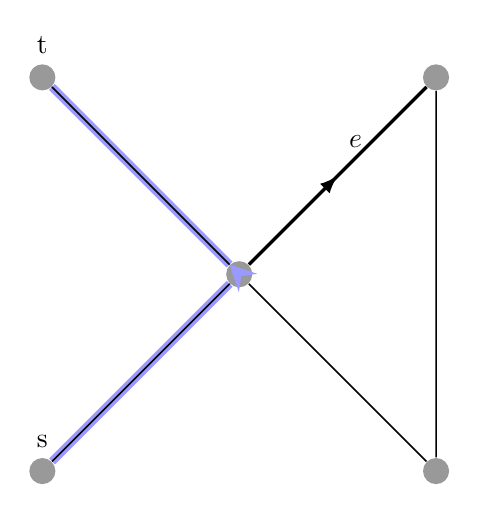
\begin{tikzpicture}
\node (s) at (0,0)[vertex, label=s]{};
% \node (stext) at (-0.1, 0.2){s};
\node (t) at (0,2)[vertex, label=t]{} ;
% \node (ttext) at (-0.1, 1.8){t};
\node (3) at (1,1)[vertex]{};
\node (4) at (2,2)[vertex]{};
\node (5) at (2,0)[vertex]{};

\draw[arcflow] (s)--(3)--(t);
\draw [edge](s) -- (3)--(5)--(4);
\draw [edge](t) -- (3);
\draw[fatarc] (3) -- (4)node [pos=0.6, above] {$e$};
\end{tikzpicture}
\caption{In the acyclic case there is no flow at all on the arc $e$ in this network}
\label{bild:acycliczeroflow}
\end{figure}

Figure \ref{bild:acycliczeroflow} shows a graph where the flow on $e$ in the acyclic case is $0$. If we do not forbid 
cyclic flows, 
the flow on $e$ will always be $\min_{a\in \textrm{ cycle }C}c_u(a)$ like in the first picture. So the gap in relative 
numbers $$ \frac{f_{cyc}(e)}{f_{acyclic}(e)}=\frac{\min_{a\in \textrm{ cycle }C}(c_u(a))}{0}$$ is not even defined!
\end{proof}

As a different relaxation we could weaken the capacity constraints, but still insist on an acyclic flow that is maximum 
on an arc $e$. In the normal Max-Flow Problem dropping the capacity constraints reduces the problem to finding a 
shortest path between the source and the sink. 

In our case, if there is only one source and one sink, we have to decide whether there is a simple path from the 
source to the sink that contains the maximized arc $e$. If there are more sources and sinks, we already have the 
problem of finding a set of simple paths containing $e$. Since the general constrained shortest path problem is 
$\mathcal{NP}$ hard this seems not to be promising and won't be disscussed here.
%TODO haerte des Problems? Wie loest man es?

%
% Is this problem easy to solve, and how to solve it? TODO
%


\subsubsection{Computational Complexity}In this chapter we will discuss the computational complexity of the \textit{Acyclic Flowbound Problem}. We show that 
Cycle-free Min-Cost-Flow with negative weights is $\mathcal{NP}$-complete, and that our problem is just a special case 
of this problem. \\

$\mathcal{NP}$-completeness is maybe the most important concept in the classification of combinatorial optimization 
problems (we will define it in a second). The $\mathcal{P-NP}$-Problem is an open question for many years now. Many 
computer scientists conjecture that in fact $\mathcal{P}\neq \mathcal{NP}$ and the $\mathcal{NP}$-complete algorithmical 
problems are hard to solve. 

The classical formal definition of the class $\mathcal{NP}$ in complexity theory uses formal languages and automata 
theory (namely Turing Machines). For this formal definition we refer to the textbook of Korte and Vygen 
\cite{KorteVygenCombOpt2007}. If we accept to be a bit less formal we can define it the following way:
\begin{definition}
%  A decision problem is an algorithmic problem that has yes or no as solution.
%  A polynomial algorithm is a procedure that 

% A combinatorial decision problem is in the complexity class $\mathcal{NP}$ if there is any nondeterministic algorithm 
% which computes the output "yes" in a polynomial number of steps.

A combinatorial decision problem (a problem with the possible solutions "yes" and "no") is in the complexity class 
$\mathcal{NP}$ iff there exists an algorithm that, given the problem and an additional input (the certificate), 
computes "yes" in a polynomial bounded number of steps if and only if the instance is a "yes"-instance of the problem 
\textit{and} the right certificate is given, otherwise false.\\
The set of problems where there exists an algorithm that always finds the correct answer in a polynomial (in the input 
size) bounded number of steps is called the complexity class $\mathcal{P}$. 
\end{definition}

Obviously all problems for which polynomial algorithms are known are in $\mathcal{NP}$, so 
$\mathcal{P}\subseteq\mathcal{NP}$. We do not know if polynomial algorithms (without the "certificate") exist for all 
problems in $\mathcal{NP}$. There are problems in $\mathcal{NP}$ for which no subexponential algorithm is known so far, 
for example the SAT problem. For some of them one can show that a polynomial algorithm for this problem already would 
imply a polynomial algorithm for all others. 

\begin{definition}
 A problem \textit{P} is called $\mathcal{NP}$-complete if \textit{P}$\in\mathcal{NP}$ and for every problem 
\textit{P'} $\in \mathcal{NP}$ there exists an algorithm with polynomial bounded running time if it can call an 
oracle for \textit{P}, i.e. a blackbox algorithm solving \textit{P} in a single step.
\end{definition}

Stephen Cook proved that every problem in $\mathcal{NP}$ can be solved by a polynomial algorithm if the SAT (boolean 
satisfiability) problem can be solved polynomially \cite{Cook:1971:CTP:800157.805047}. 
Richard Karp presented the result that the hamiltonian cycle problem (and by this also the hamiltonian path problem) 
can be reduced to SAT (\cite{Karp1972}). Thus these problems are $\mathcal{NP}$-complete.

We want to show that the acyclic minimum cost flow problem, of which the acyclic flowbound problem is a special case, 
is an $\mathcal{NP}$-complete problem. This justifies to deal with algorithms that either are not provable to have 
polynomial worst case running time or else are no exact algorithms but rather heuristics to find a weaker bound.


%TODO kann man für das Unterproblem selbst auch etwas zeigen? Das 
%könnte ja durchaus auch Polynomiell sein!

\begin{definition}
 We call the problem of finding a Minimum Cost Flow as in Definition \ref{def:mincostflow} in a given 
network $G$ with the additional constraint  that there is no cyclic flow the \textit{Acyclic Minimum Cost Flow} 
Problem. 

The corresponding decision problem is to decide the question if there can be any acyclic flow with total cost of at 
most $x$ in the network. With binary search on the values of $x$ we can solve any optimization problem by iteratively 
solving the corresponding decision problem - so since both have the same complexity, we can speak of $\mathcal{NP}$ 
completeness of the optimization problem as well . 
\end{definition}

\begin{theorem}
 The \textit{Acyclic Minimum Cost Flow Problem} with arbitrary arc weights is $\mathcal{NP}$ complete.
\end{theorem}
\begin{proof}
 We have to show two things: The problem is in the complexity class $\mathcal{NP}$ , and the problem is indeed 
$\mathcal{NP}$ hard. We do this via two lemmas:
\begin{lemma}
 The Acyclic Minimum Cost Flow Problem is in the complexity class $\mathcal{NP}$
\end{lemma}
\begin{proof}
It is easy to see that the problem is in $\mathcal{NP}$. Given a valid solution to the decision problem we can check if 
it is a feasible network flow by just checking the flow balances on all nodes, which needs only linear time 
$\mathcal{O}(|V|+|A|)$. We can also easily check if the total cost is smaller or equal than demanded and that all 
capacities are respected by running over all arcs and checking them, thus this part is also linear.
We can also check the acyclicity in polynomial time: On each of the arcs we can start a graph search, considering arcs 
only in their flow direction. If this graph search comes back to the original arc again, there is a cycle. %TODOprove?
If graph search does not find a way to the tail of the original arc, there is no cyclic flow on this arc. The graph 
search is also a linear algorithm. If we do this for each arc, the running time is still quadratic.
\end{proof}

\begin{lemma}
 The Acyclic Minimum Cost Flow Problem is $\mathcal{NP}$-hard.
\end{lemma}
\begin{proof}

To show the $\mathcal{NP}$ hardness, we reduce the problem to the \textit{undirected $s-t$-Hamiltonian Path Problem} 
which is well known as a standard example for $\mathcal{NP}$ completeness. Hamiltonian cycle is $\mathcal{NP}$ 
complete both in the directed and undirected case, see \cite{Karp1972}. To find an $s-t$-hamiltonian path in a graph 
$G$ for some vertices $s,t\in V(G)$ we add one extra vertex $x$ and the edges $(t,x)$ and $(x,u)$ to $G$. This new 
graph has a hamiltonian cycle if and only if $G$ has a hamiltonian path from $s$ to $t$. \\
%done zitieren wo hampath vorkommt,NP-haertebeweis

Given an instance of the $s-t$-Hamiltonian Path problem, we have to transform it into an instance of our problem. Then 
we show that the reduced problem is a yes-instance of the Acyclic Min Cost Flow decision problem if and only if the 
original instance of the Hamiltonian Path problem is a yes-instance. Further the reduction must be computable in 
polynomial time.
 
\begin{figure}[h!]
\centering
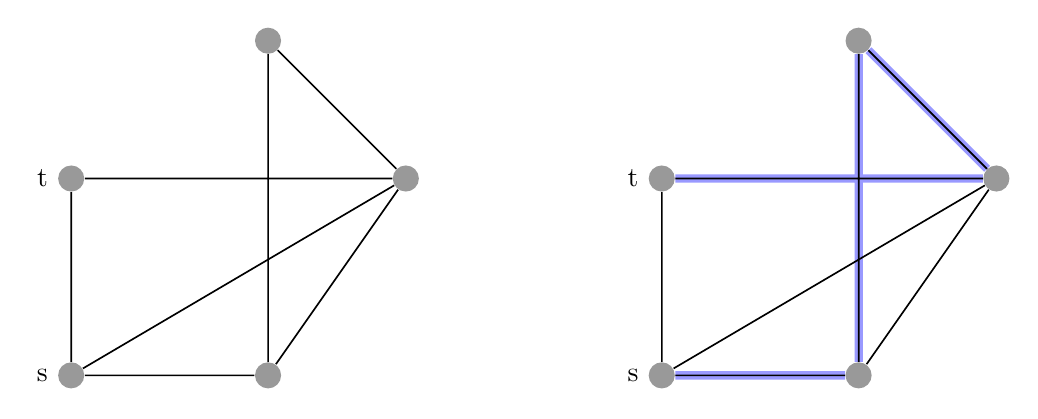
\begin{tikzpicture}
\node (s) at (0,0)[vertex, label=left:s]{};
\node (t) at (0,1)[vertex, label=left:t]{} ;
\node (3) at (1,0)[vertex]{};
\node (4) at (1,1.7)[vertex]{};
\node (5) at (1.7,1)[vertex]{};

% \draw[edgeflow] (s)--(3)--(4)--(5)--(t);
\draw[edge] (s)--(3)--(4)--(5)--(t);
\draw[edge] (t)--(s)--(5)--(3);

%now draw the transformed graph
\node (s2) at (3,0)[vertex, label=left:s]{};
\node (t2) at (3,1)[vertex, label=left:t]{} ;
\node (32) at (4,0)[vertex]{};
\node (42) at (4,1.7)[vertex]{};
\node (52) at (4.7,1)[vertex]{};

\draw[edgeflow] (s2)--(32)--(42)--(52)--(t2);
\draw[edge] (s2)--(32)--(42)--(52)--(t2);
\draw[edge] (t2)--(s2)--(52)--(32);
\end{tikzpicture}
\caption{This graph has an $s-t$-hamilton path contained, marked in blue in the second picture}
\label{bild:hampath}
\end{figure}

An $s-t$-Hamiltonian Path is a path in a network starting at node $s$ and ending at node $t$ that is visiting every 
node of $G$ exactly once like in the example in figure \ref{bild:hampath}. 

This can only work in connected graphs, so we know that if $n$ is the number of nodes in the 
graph, the Hamiltonian Path has to have size $n-1$. Our reduction is the following:

Transform the $s-t$-Hamiltonian Path instance into an instance of a flow network where for each edge $\{uv\}$ there 
are two directed arcs $(u,v),(v,u)$, the arcs $a\in A$ all have capacities $c(a)=[0,1]$ and costs of $-1$ 
with the same underlying graph as before. The nodes $s$ and $t$ become the source and sink of the flow.
The decision we ask for is whether there is a flow with total costs of at most $-(n-1)$ or not. (Figure 
\ref{bild:hampathreduct} shows an example of such a transformation)

 
\begin{figure}[h!]
\centering
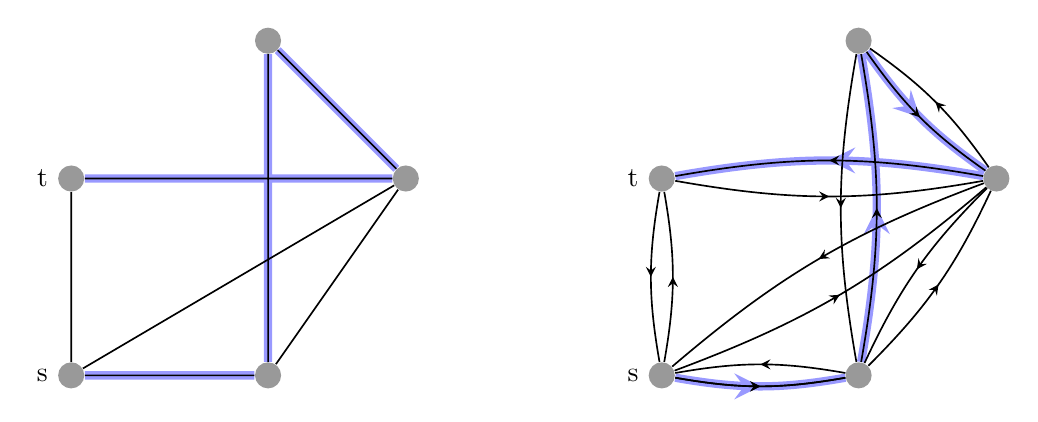
\begin{tikzpicture}
\node (s) at (0,0)[vertex, label=left:s]{};
\node (t) at (0,1)[vertex, label=left:t]{} ;
\node (3) at (1,0)[vertex]{};
\node (4) at (1,1.7)[vertex]{};
\node (5) at (1.7,1)[vertex]{};

\draw[edgeflow] (s)--(3)--(4)--(5)--(t);
\draw[edge] (s)--(3)--(4)--(5)--(t);
\draw[edge] (t)--(s)--(5)--(3);

%now draw the transformed graph
\node (s2) at (3,0)[vertex, label=left:s]{};
\node (t2) at (3,1)[vertex, label=left:t]{} ;
\node (32) at (4,0)[vertex]{};
\node (42) at (4,1.7)[vertex]{};
\node (52) at (4.7,1)[vertex]{};

\draw[curvedarcflow](s2)to(32);
\draw[curvedarcflow](32)to(42);
\draw[curvedarcflow](42)to(52);
\draw[curvedarcflow](52)to(t2);
\draw[curvedarc](s2)to(32);
\draw[curvedarc](32)to(s2);
\draw[curvedarc](42)to(32);
\draw[curvedarc](32)to(42);
\draw[curvedarc](42)to(52);
\draw[curvedarc](52)to(42);
\draw[curvedarc](t2)to(52);
\draw[curvedarc](52)to(t2);
\draw[curvedarc](s2)to(32);
\draw[curvedarc](s2)to(52);
\draw[curvedarc](52)to(s2);
\draw[curvedarc](52)to(32);
\draw[curvedarc](32)to(52);
\draw[curvedarc](t2)to(s2);
\draw[curvedarc](s2)to(t2);

\end{tikzpicture}
\caption{A graph with an $s-t$-hamilton path is transformed to an acyclic minimum cost flow instance with costs of $-1$ 
per arc. Hence in this example we find a minimum acyclic flow of cost $-4=-n+1$}
\label{bild:hampathreduct}
\end{figure}

It is obviously a polynomial time transformation because only a linear number of flags and arcs is added to the 
network, while the edges are deleted when they get replaced with the new arcs.

It yields the same decision as the original Hamiltonian Path instance:
\begin{itemize}
 \item $\Rightarrow:$ Given an instance of the Acyclic Min Cost Flow which has a acyclic flow from $s$ to $t$ with cost 
$-n+1$.
Flow can have a value of at most $1$ on each arc, so each arc the flow is going through can only contribute up to $-1$ 
costs to the cost function. The flow could be split up into different paths from $s$ to $t$, but we know that there are 
no cycles. That means on every of these paths every node is visited only once - if we see it twice we have closed a 
cycle. The cost of the flow is minus the average length of the paths of flow. So we can conclude there is at least one 
path with length $n-1$ that is seeing no node twice - hence it has to see every node exactly once, so we found (at 
least) one $s-t$-Hamiltonian Path and know it is a yes-instance of Hamiltonian Path too.

\item $\Leftarrow:$ Given a graph together with an $s-t$-Hamiltonian Path. In the transformed instance of Min Cost Flow 
we get immediately a feasible $s-t$-Flow by setting the flow value on all forward arcs on the given hamiltonian path 
equals $1$. This flow also has total costs of $-(n-1)$.
\end{itemize}
\end{proof}

These two lemmas together show that our problem of finding an acyclic flow with minimum costs and arbitrary weight 
function is in general $\mathcal{NP}$-complete.
\end{proof}

\newpage
\section{Models and Solving Approaches}%main section about the different models 
In this section we describe different mathematical models that can be used to obtain bounds on the acyclic flow going 
over a specified arc of the given flow network (assumed there is any feasible network flow). We present two different 
MIP models of the acyclic flowbound problem. The first model uses node potentials and constraints to force flow to 
go in direction from higher to lower potentials. The second model uses decision variables for the direction of the 
flow and special acyclicity constraints on them for each cycle. They are different in size as the second MIP model 
explicitly uses constraints on the cycles to exclude cyclic flow from the solution. We show that it is not sufficient 
to have these constraints just on a cycle base (which would be a linearly small number). But we can prove 
conditions under which the acyclicity constraint of a cycle becomes redundant. Still there can be exponential many 
cycles in a network and the condition could be fulfilled on \textit{cycle} of the network. 

Furthermore we discuss an idea to solve the problem with a direct algorithm augmenting paths. We show by examples that 
path augmentation alone can not solve the problem, but the idea inspires a relaxation/heuristic algorithm which runs in 
polynomial time.


\subsection{MIP Formulations}
For many combinatorial Problems it is the best practical solution to formulate them as a Mixed Integer Problem and just 
solve this problem with modern MIP Solvers such as CPlex, Gurobi, SCIP etc. Often there are different possible 
formulations of the problem as 
MIP, which might yield very different running times due to numerical or algorithmical reasons. In our problem, it is 
easy to model the flow conservation and the ingoing and outgoing flow on vertices. Like described before, we can assign 
a negative weight to an arc variable and this way maximize flow over this arc by minimizing the overall cost. This 
would be the typical MIP formulation of a min cost flow:

\begin{align*}
  &\min \sum_{a\in A} w_a\cdot q_a  \\
  %TODO an die balance-intervall formulierung anpassen
 s.t. & \sum_{a\in \delta^+(v)}q_a - \sum_{a\in\delta^- (v)}q_a = d_v\ &\forall v\in V \\
  & c_l(a)\le q_a \le c_u(a) & \forall a\in A
\end{align*}

This model still allows cyclic flow, so we have to find constraints to avoid cyclicity. 
\subsubsection{Model 1: Node Potentials}
\label{model:nodePotential}
%TODO welche formulierungen koennte es noch geben fuer dieses problem?
%TODO PORTA results and polytope of the problem?

One idea (that is unfortunately not a linear problem formulation anymore) would be to set potentials on the nodes and 
allow only flow from higher to lower potential. This is quite close to the application of our problem in gas flow 
computation, where gas will only flow from places with high pressure to places with lower pressure in the network. So 
each vertex $v$ would get a variable $\pi_v$ for its potential, each arc $a$ as before a variable $q_a$ for the amount 
of flow. Then we add the constraint $$q_a\cdot (\pi_v -\pi_w)\ge 0\,\forall a=(v,w)\in A $$
We have to ensure that the values of the potentials are all 
different, or that there is no flow between nodes of the same potential. Otherwise any solution where all potentials 
are set to the same value would fulfill this constraint, regardless if it is acyclic or not. So in practice we could 
set a constant $\varepsilon > 0$ to describe the minimum distance between the potentials. A feasible 
solution now has to fulfill the constraint above on every arc. If we set up the constraint as above, we get the Mixed 
Integer Nonlinear Program

\begin{align*}\label{model:nodePotentialQuadratic}
  &\min \sum_{a\in A} w_a\cdot q_a & \\
 s.t. & \sum_{a\in \delta^+(v)}q_a - \sum_{a\in\delta^- (v)}q_a &=& d_v\ &\forall v\in V \\
 & q_a &\le& c_u(a) & \forall a\in A\\
 & -q_a &\le& c_l(a) & \forall a\in A\\
 & -q_a\cdot (\pi_v -\pi_w)&\le& 0 &\forall a=(v,w)\in A\\
 & (\pi_v - \pi_w)^2 &\ge& \varepsilon &\forall v,w \in V\\
 & q_a \in \R & & &\forall a\in A\\
 & \pi_v \in \R & & & \forall v\in V\\
 & d_a \in \{0,1\} & & &\forall a\in A\\
\end{align*}

We show that this flow indeed is an acyclic one:

\begin{prop}
 A flow which fulfills the constraints of the above nonlinear program is always acyclic.
\end{prop}
\begin{proof}
 Assume a flow fulfilling the above constraints would have cyclic flow on a cycle $C$. Without loss of generality 
we label the vertices on the cycle from $1$ to $n$ and assume all arcs are directed forward on this cycle. This means 
there are arcs $a_1=(v_1,v_2),a_2=(v_2,v_3), \dots a_n=(v_n, v_1)\in C$ such that $q_{a_i} > 0 \,\forall i={1,\dots , 
n}$. Also we know from the constraints  $q_a\cdot (\pi_v -\pi_w)\ge 0$ and $\pi_v - \pi_w \neq 0$ (Hence $\Rightarrow 
\pi_v\neq\pi_w)\, \forall v,w\in V$. So we conclude an ordering of the vertices potentials: $q_{a_1}\cdot (\pi_{v_1} 
-\pi_{v_2})\ge 0 \Rightarrow \pi_{v_1}>\pi_{v_2}$ and so on. This yields a sequence $\pi_{v_1}>\pi_{v_2}>\dots 
>\pi_{v_n}>\pi_{v_1}$, which is a contradiction. \Lightning
\end{proof}

However, solving nonlinear mixed integer programs comes with many difficulties, so we will use indicator constraints 
or an equivalent Big-M constraint to get a mixed integer formulation avoiding these difficulties. For this we  replace 
$$q_a\cdot (\pi_w -\pi_v)\le 0 \,\forall a=(v,w)\in A $$ and $$(\pi_v - \pi_w)^2 \ge \varepsilon \,\forall v,w \in V$$

%introduce rho (=richtung) variables
Instead we introduce a new binary variable $\rho_{vw}$ to indicate the flow direction on $a=(v,w)$, and say this 
variable has to be 1 if flow is from $v$ to $w$ and 0 if it is from $w$ to $v$. Also if $\rho_{vw}$ is $1$ the 
potential $\pi_v$ of $v$ has to be greater than the potential $\pi_w$ of $w$ and the other way around. So with 
indicatorconstraints we get 

% \label{model:nodePotentialIndicator}
\begin{align*}
 &\rho_{vw}=1 &\Rightarrow &\pi_v\ge\pi_w +1\\
 &\rho_{vw}=0 &\Rightarrow &\pi_w\ge\pi_v +1\\
 &\rho_{vw}=1 &\Rightarrow &q((v,w))\ge 0\\
 &\rho_{vw}=0 &\Rightarrow &q((v,w))\le 0\\
 &\rho_{vw} \in \{0,1\}&&
\end{align*}
We can reformulate these indicator constraints as

%  \label{model:nodePotentialBigM}
\begin{align*}
 &\pi_v-\pi_w &\ge & N(\rho_{vw}-1)+1\\
 &\pi_v-\pi_w&\le &N\rho_{vw}-1 \\
 &q((v,w))&\ge& M(\rho_{vw}-1)\\
 &q((v,w))&\le & M\rho_{vw}\\
 &\rho_{vw} \in \{0,1\}&&\\
\end{align*}
where $N\in \R$ and $M\in \R$ are sufficient big constants. Sufficient big in this case could mean we choose 
$N=|V|\, ,M=\sum_{v\in V}|d(v)|$. \\
So the complete Mixed Integer Program is:

% \label{model:nodePotentialWithBigM}
\begin{align*}
  &\min \sum_{a\in A} w_a\cdot q_a & \\
 s.t. & \sum_{a\in \delta^+(v)}q_a - \sum_{a\in\delta^- (v)}q_a &=& d_v\ &\forall v\in V \\
 & q_a &\le& c_u(a) & \forall a\in A\\
 & q_a &\ge& c_l(a) & \forall a\in A\\
 & \pi_v-\pi_w &\ge & N(\rho_{vw}-1)+1& \forall a=(v,w)\in A\\
 & \pi_v-\pi_w&\le &N\rho_{vw}-1& \forall a=(v,w)\in A\\
 & q_a&\ge& M(\rho_{vw}-1)& \forall a=(v,w)\in A\\
 & q_a&\le & M\rho_{vw}& \forall a=(v,w)\in A\\
 & q_a \in \R & & &\forall a\in A\\
 & \pi_v \in \R & & & \forall v\in V\\
 & d_a \in \{0,1\} & & &\forall a\in A\\
 & \rho_{vw} \in \{0,1\}&&& \forall a=(v,w)\in A\\
\end{align*}
%TODO show that these constraints are equivalent to the nonlinear ones? or make a comment at least?

\subsubsection{Model 2: Acyclicity Constraints On All Cycles}
\label{model:AcyclicityConstraints}
Another idea to solve the Acyclic Flow Bound Problem 
%(which was partially implemented in Lamatto by Robert Schwarz) 
is the following: Every arc has a direction and the 
sign of the flow on this arc tells us in which direction flow is send over this arc. Again we introduce variables 
$\rho_a\in \{0,1\}$ for each arc $a\in A$ that indicate the direction of flow and are coupled with the flow variables:
\begin{align*}
\rho_a=1 & \Rightarrow q_a\ge 0 \\
\rho_a=0 & \Rightarrow q_a\le 0
\end{align*}
These indicator constraints can be handled the way they are by standard MIP solvers, but to make them real MIP 
constraints we may formulate them as follows (with $M$ a constant sufficient big, e.g. $M=\sum_{v\in V}|d_v|$) :
\begin{align*}
 q_a + M\cdot (1-\rho_a) &\ge 0\\
 q_a - M\cdot \rho_a & \le 0
\end{align*}

In addition to decision variables for the flow direction, we have to add constraints to avoid cycles. If the flow is 
acyclic, each cycle should have at least two arcs with opposite directions. In other words, there has to be one arc
in forward direction and one in backward direction, so with $n:=|C|$ we get as constraint:
$$ 1\le\sum_{a\in C\textrm{ forward }} \rho_a + \sum_{a\in C\textrm{ backward }}1-\rho_a\le n-1$$

Let us formulate this in a slightly different way to get only one sum: For each cycle of size $C_n=C_l+C_m$ 
let $C_m$ be the number of arcs directed forward and $C_l$ the number of arcs directed backward. We define that always 
$C_l\le C_m$, so forward is defined as the direction that more arcs are pointing towards (left or right would only 
make sense in a planar embedding). Then we get the constraint $$1-l \le \sum_{a\in C}\rho_a\le n-(l+1)$$ that forbids 
any cyclic flow on $C$. We will show later under which conditions such constraints also forbid cyclic flow on other 
cycles. 
%TODO was ist wenn gleich viele? Ist das als Definition so ueberhaupt ok?

So our MIP formulation of the model is finally
\begin{align*}
 &\min \sum_{a\in A} w_a\cdot q_a & \\
 s.t. & \sum_{a\in \delta^+(v)}q_a - \sum_{a\in\delta^- (v)}q_a = d_v\ &\forall v\in V \\
  & c_l(a)\le q_a \le c_u(a) & \forall a\in A\\
 &q_a + M\cdot (1-\rho_a) \ge 0 & \forall a\in A\\
 &q_a - M\cdot \rho_a \le 0 & \forall a\in A\\
 &1-l \le \sum_{a\in C}\rho_a \le n-(l+1) & \forall \textrm{ cycle }C\in G\\
 & q_a \in \R &\forall a\in A\\
 & \rho_a \in \{0,1\} &\forall a\in A
\end{align*}
or if we normalize the MIP to only $\le$ inequalities:
\begin{align}
 &\min \sum_{a\in A} w_a\cdot q_a & \\
 s.t. & \sum_{a\in \delta^+(v)}q_a - \sum_{a\in\delta^- (v)}q_a &=& b_v\ &\forall v\in V \\
 & q_a &\le& c_u(a) & \forall a\in A\\
 & -q_a &\le& c_l(a) & \forall a\in A\\
 &-q_a - M\cdot (1-\rho_a) &\le& 0 & \forall a\in A\\
 &q_a - M\cdot \rho_a &\le& 0 & \forall a\in A\\
 &1-l - \sum_{a\in C}\rho_a &\le& 0 & \forall \textrm{ cycle }C\in G\\
 & \sum_{a\in C}\rho_a +(l+1)-n &\le& 0 & \forall \textrm{ cycle }C\in G\\
 & q_a \in \R & & &\forall a\in A\\
 & \rho_a \in \{0,1\} & & &\forall a\in A
\end{align}


\subsection{The number of cycles we have to forbid}
The model above has one obvious problem we have to deal with: Since it has a constraint for every cycle of $G$ and the 
number of cycles in a graph might be exponential, even setting up the model would need exponential running time. 

So do we really need every cycle? Or is it enough to just forbid cyclic flow on a small subset (e.g. a cycle base) of 
the cycles of $G$? 

The figures \ref{bild:reichtkreisbasis1} and \ref{bild:reichtkreisbasis2} %TODO
show that a cycle base works on the easiest possible example, but fails if the problem gets just a bit more complicated:

%Bild/bsp: zwei dreiecke mit einer gemeinsamen seite - auf 2 Kreisen Fluss verbieten reicht TODO
\begin{figure}[h!]
\centering
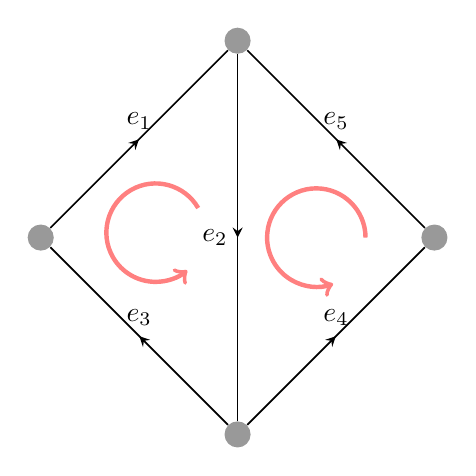
\begin{tikzpicture}
\node (a) at (0,0)[vertex]{};
% \node () at (-0.1, 0.2){};
\node (b) at (1,1)[vertex]{} ;
\node (c) at (1,-1)[vertex]{};
\node (d) at (2,0)[vertex]{};

\draw[arc] (a) -- (b)node [pos=0.5, above]{$e_1$};
\draw[arc] (b) -- (c)node [pos=0.5, left]{$e_2$};
\draw[arc] (c) -- (a)node [pos=0.5, above]{$e_3$};
\draw[arc] (c) -- (d)node [pos=0.5, above]{$e_4$};
\draw[arc] (d) -- (b)node [pos=0.5,above]{$e_5$};
%draw circle with arrowtip
\draw[ultra thick, ->, red!50] (1.65,0) arc (0:290:0.25);
\draw[ultra thick, ->, red!50] (0.8,0.15) arc (30:310:0.25);
\end{tikzpicture}
\caption{Here it suffices to forbid the 2 interior cycles marked with red in order to obtain acyclicity}
\label{bild:reichtkreisbasis1}
\end{figure}
%beweis dass hier wirklich eine Kreisbasis reicht!

Why are the constraints of a cycle base sufficient in this case of figure \ref{bild:reichtkreisbasis1}? 

We see this immediately, when we look at all acyclicity constraints for the 3 cycles contained in the graph:
\begin{align*}
 1 &\le x_1+x_4+x_5\le 2&\\
 1&\le x_2+x_3+x_5\le 2& \iff -2\le -x_2-x_3-x_5\le -1\\
 -1 &\le x_1-x_2-x_3+x_4 \le 1&
\end{align*}
The last inequality is exactly the sum of the two inequalities above. Hence if two are fulfilled, the last one is 
automatically induced by them, it is a redundant constraint.

%BILD : bei einem ``tetraeder''-graphen reicht es nicht, drei der möglichen Kreise zu verbieten!
\begin{figure}[h!]
\centering
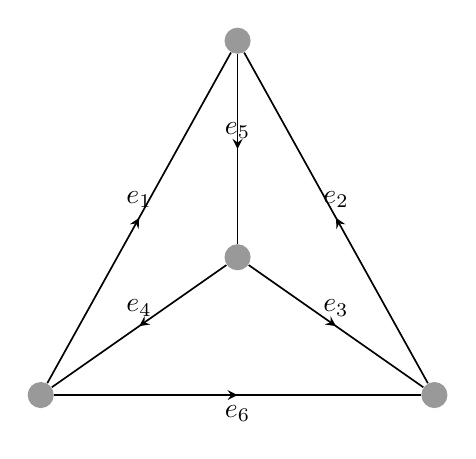
\begin{tikzpicture}
\node (a) at (0,-0.1)[vertex]{};%center 
\node (b) at (-1,-0.8)[vertex]{} ;
\node (c) at (0,1)[vertex]{};
\node (d) at (1,-0.8)[vertex]{};
% \node(etext) at (1.4,1.6){e};

\draw[arc] (a) -- (b)node [pos=0.5, above]{$e_4$};
\draw[arc] (b) -- (c)node [pos=0.5, above]{$e_1$};
\draw[arc] (c) -- (a)node [pos=0.5, above]{$e_5$};
\draw[arc] (a) -- (d)node [pos=0.5, above]{$e_3$};
\draw[arc] (d) -- (c)node [pos=0.5, above]{$e_2$};
\draw[arc] (b) -- (d)node [pos=0.5, below]{$e_6$};
\end{tikzpicture}
\caption{In this tetrahedron graph \textbf{no} cycle bases' acyclicity constraints can enforce acyclic flow on the 
whole 
graph}
 \label{bild:reichtkreisbasis2}
\end{figure}
For figure \ref{bild:reichtkreisbasis2} the situation is more complex, though there is only one more arc in the graph. 
But the number of cycles grows exponentially, so we get 7 cycles in this case. Their inequalities are:
\begin{align*}
 1 &\le x_1+x_4+x_5\le 2&\\
 1&\le x_2+x_3+x_5\le 2& \\%\iff -2\le -x_2-x_3-x_5\le -1\\
 -1&\le x_3-x_4-x_6\le 0\\
 -1&\le x_1-x_2-x_6\le 0\\ 
 -1 &\le x_1-x_2-x_3+x_4 \le 1&\\
 0 &\le x_1+x_3+x_5-x_6\le 2\\
 1&\le x_2+x_4+x_5+x_6\le 3\\
\end{align*}
We could choose the three cycles $(e_1 e_5 e_4)$, $(e_2 e_5 e_3)$, $(e_3 \overline{e_6}\, \overline{e_4})$ as a cycle 
base, these cycles induce the first three constraints. By combining the first and second, we directly get the fifth 
inequality $-1 \le x_1-x_2-x_3+x_4 \le 1$ as above (this one is of course still redundant). But if we add inequality 
$3$, the result is 
\begin{align*}
 &&-1 &\le &x_1&-x_2&-x_3&+x_4 &&\le 1\\
 &+&-1&\le &&&x_3&-x_4&-x_6&\le 0\\
 &=&-2&\le&x_1&-x_2&&&-x_6&\le 1
\end{align*}
But the acylicity constraint of the cycle $(e_1 \overline{e_2} \,\overline{e_6})$ is $-1\le x_1-x_2-x_6\le 0$ instead. 
The resulting constraints are not sharp, because the left hand side and the right hand side depend on the length of the 
cycles, which changes while we combine them.

Due to symmetry in this complete graph it does not matter which cycles we choose for the cycle base. In fact there is 
no combination of three cycles that could completely exclude cyclic flow solutions from the solution space.

\begin{prop}
\label{prop:redundantAcyclicityCons}
 Given two acyclicity constraints $cons_1$ and $cons_2$ of cycles $C_1$ and $C_2$ in $G$. The acyclicity constraint of 
the joint cycle $C=C_1\cup C_2 \setminus \{a\in A| a\in C_1\land a\in C_2 \}$ is the sum of $cons_1$ amd $cons_2$ if 
and only if $C_1$ and $C_2$ have exactly one arc in common (and this arc is directed differently in both 
cycles/has different sign in both constraints).
\end{prop}
This proposition shows that many of the acyclicity constraints in our model may be redundant and could be omitted. 
But still the remaining constraints are exponential in the size of $G$.

\begin{proof}
 Assume we are given two cycles $C_1,\,C_2\in G=(V,A)$ with exactly one arc $g\in A$ 
contained in both cycles, and the direction of the cycles such that $g$ is forward in one cycle and backward in the 
other cycle. Without loss of generality we assume it is forward in $C_1$ and backward in $C_2$, i.e. $x_g$ has a 
positive sign in $cons_1:\,lhs_1\le \dots\le rhs_1$ and a negative sign in $cons_2:\, lhs_2\le \dots\le rhs_2$, which 
are the acyclicity constraints of $C_1$ and $C_2$. 

$\Rightarrow :$ 
The acyclicity constraints $lhs \le \dots\le rhs$ are constructed such that always $rhs-lhs=l-2$, $l$ being the length 
of the cycle the constraint belongs to. Consider two cycles $C_1$ and $C_2$ and let $J\subset A=\{a\in A|a\in C_1 
\land a\in C_2 \}$ be the set of arcs that are contained in both cycles, $j:=|J|$. 

If we sum up the constraints $cons_1$ and $cons_2$ of the cycles $C_1$ and $C_2$ we obviously get another constraint,
say $cons_3:\, lhs=lhs_1+lhs_2\le\dots\le rhs_1+rhs_2=rhs$. The length of the joint cycle $C$ is $l=l_1+l_2-2\cdot j$. 
We have 
$$rhs-lhs=rhs_1+rhs_2-lhs_1-lhs_2=\underbrace{rhs_1-lhs_1}_{l_1-2}+\underbrace{rhs_2-lhs_2}_{l_2-2}=l_1+l_2-4$$
It holds
$$l_1+l_2-4=l_1+l_2-2j-2=l-2 \iff j=1$$ 
This means that only if $C_1$ and $C_2$ have exactly one arc in common (i.e. $j=1$), the necessary condition 
$rhs-lhs=l-2$ is fulfilled to get the new acyclicity constraint.

$\Leftarrow :$ Now we have to show that we get a sharp acyclicity constraint every time we sum up two acyclicity 
constraints that have exactly one variable in common, and this has different sign in both constraints (so it cancels 
out). Let $cons_1$ and $cons_2$ be chosen this way and $C_3=C_1\cup C_2\setminus (C_1\cap C_2)$ be the resulting cycle, 
then we get:
\begin{align*}
 &&1&\le &\sum_{a \textrm{ forward in }C_1}q_a + \sum_{a\textrm{ backward in }C_1}{(1-q_a)}&&\le &l_1-1\\
 &+&1&\le &\sum_{a \textrm{ forward in }C_2}q_a + \sum_{a\textrm{ backward in }C_2}{(1-q_a)}&&\le &l_1-1\\
 &=&2&\le &\sum_{a \textrm{ forward in }C_3}q_a +\sum_{a\textrm{ backward in }C_3}{(1-q_a)}+
 &\underbrace{q_a+1-q_a}_{a\in C_1\cap C_2} &\le &l_1+l_2-2\\
 \iff &&1&\le &\sum_{a \textrm{ forward in }C_3}q_a +\sum_{a\textrm{ backward in }C_3}{(1-q_a)}
 &&\le &\underbrace{l_1+l_2-2}_{l_3}-1\\
\end{align*}
which is exactly the acyclicity constraint of the cycle $C_3$.
\end{proof}
%other redundant constraints: if in the middle there is no source or sink
There are still more redundant acyclicity constraints than these. Under certain conditions the acyclicity of smaller 
cycles implies the acyclicity of combined cycles even if there is more than one arc contained in both cycles.

\begin{prop}
 Given two cycles $C_1, C_2$ with a set of shared arcs $J:=\{a\in C_1|a\in C_2\}$ which we assume to have size greater 
than one ($j:=|J|>1$). If $J$ is a path in the graph with no sink or source vertex in the interior, the acyclicity of 
$C_1, C_2$ together implies acyclicity of the cycle $C_3:=C_1\cup C_2\setminus C_1\cap C_2$.
\end{prop}
\begin{proof}
 We prove this via contradiction. If the common arcs $J$ are a path like above, they have flow always in the same 
direction. Suppose $C_1$ and $C_2$ are acyclic, but $C_3$ is not. This means in both $C_1$ and $C_2$ there are arcs 
with different directions on the cycle, while they are all in the same direction on $C_3$. This means, the arcs with 
different direction have to be in the path $J$ of shared arcs of $C_1$ and $C_2$. Hence within the path $J$ there must 
be arcs which are directed oppositely to each other. This can only happen, if one of the vertices in the interior of 
$J$ is a sink or a source. \Lightning
\end{proof}
%verallgemeinerung: teilt ein kreis den graph in zwei teile, dann ist es ausreichend wenn im innern azyklizität gegeben 
%und keine quelle/senke vorhanden ist? (verallgemeinerung von planarem Fall)
We can prove something more general by giving conditions that apply in more cases:
\begin{prop}
 Given a graph $G=(V,A)$ , without loss of generality assumed to be connected, and a cycle $C\subset G$ with the 
following properties:
 \begin{itemize}
  \item $G\setminus C$ is disconnected
  \item Let $G'$ be a connected component of $G\setminus C$ 
  \item $G'$ has no source or sink nodes
  \item $G'\cup C$ consists of cycles whose direct sum is $C$ %TODO is direct sum what I really mean? Define it?
 \end{itemize}
 Then any acyclic orientation of the other cycles than $C$ in $G'\cup C$ implies already the acyclicity of $C$. This 
  means the acyclicity constraint of $C$ is redundant.

\end{prop}
%Beweisen, dass in einem Gebiet ohne Quellen oder Senken (das planar ist?) einfache kreise reichen
\begin{proof}
 Consider only the subgraph $G'\cup C$ and assume $C$ had a cyclic orientation. In $C$ there has to be a chordal path 
through $G'$. Since there are no sources or sinks in $G'$, in fact there must be a \textit{directed} path from one node 
$v_1 \in C$ to another node $v_k\in C$ going through $G'$: starting from any arc incident to a node on $C$ and one in 
$G'$, we will always find another arc from the endnode in the same direction unless we run into a cycle or a 
source/sink node. But since neither exists in $G'$, after a finite number of arcs we come to a node on $C$ again. Thus 
we can always find a directed path in our setting. 

But there are two smaller cycles $C_1$ and $C_2$ if we divide $C$ along this path. $C$ is a directed cycle and the path 
is also directed $\Rightarrow$ so one of the two cycles has to be directed, which contradicts our assumption. 
\Lightning 

Hence we conclude that acyclicity and absence of sources/sinks in the interior of a cycle make its acyclicity 
constraint redundant.
\end{proof}

%remark that this more general proposition is important for the planar case
There are some special cases where the above result can be very helpful and indeed reduce the number of needed 
acylicity constraints to polynomial size. This is not only relevant in theory, but also in practice: a real world gas 
network might have (at least partially) a planar graph representation. Planar graphs fulfill the condition to find a 
cycle which is dividing the graph into different parts easily - each cycle in a planar graph embedding divides the 
graph 
into interior and exterior. If we have only one source and one sink and find an embedding where both are on the outer 
(unbounded) face of the graph, it is sufficient to have the acyclicity constraints only on the face cycles of the 
graph. The same holds for all areas or subgraphs without sources/sinks that are enclosed by a cycle: we only need small 
simple cycles and all other acyclicity constraints are redundant.

% TODO BILD : Bei einem Gitter mit vielen Quellen/Senken sind wir verloren... !
Still we have a problem with the sources and sinks. If there are many of them we still run into exponential numbers of 
acyclicity constraints.

\newpage
\subsection{The Constrained Path Augmentation Model}%TODO kann man so ein modell finden, das mithilfe von constrained 
% shortestpath problemen einen successive shortest path algo zu einem maxflowbound-algo macht? duerfte schwer werden...
\label{model:pathaugment}
The main idea in this chapter was to design an algorithm that uses path augmentation to saturate the given flow 
demands. 
The algorithm should try to push as much flow value as possible over the arc where flow is maximized, while having the 
constraint that the resulting flow is acyclic. %TODO geht das ueberhaupt mit succ shortest path?
Algorithms that use path augmentation to compute flows are well known and among the standard flow algorithms. The 
algorithm of Ford and Fulkerson \cite{Ford-Fulkerson_algo} arising from their Max-Flow-Min-Cut theorem is based on 
source-sink-paths in the network as well as the improved algorithms of Edmonds and Karp \cite{EdmondsKarp1972} or Dinic 
\cite{Dinic1970}. 

This idea of path augmentation is conveniant and nice looking in the beginning. It is the base for a direct heuristic 
approach to the problem that can produce valid bounds very fast. We also show the difficulties of choosing a path and 
illustrate with examples that only a relaxed version or either an algorithm with edge progressions instead of simple 
paths can work for the acyclic flowbound problem.\\

If we want to maximize flow over arc $e=(u,v)$ the first idea might be to just search a path from $v$ to the sink $t$ 
and another path from the sink $s$ to $u$. Finding such a path can be done by graph search in the graph of augmentable 
arcs in linear time. Also the combined path of the two would always use the arc $e$.
But it is not sufficient to just combine a path from source $s$ to node 
$u$ and one from node $v$ to a sink $t$. Such a combination could produce cyclic flow, see for example figure 
\ref{bild:cycleFromCombinedPaths}. %TODO BILD

%Bild: combining two paths can produce a cycle TODO noch verbessern... z.b. kreis mit einem loop markieren
\begin{figure}[h!]
\centering
\begin{tikzpicture}
% [scale=2, vertex/.style={circle,fill=black},arrow/.style={-latex, shorten >=0.2ex, shorten <=0.2ex}]
\node (a) at (2,0)[vertex, label=below:$v$]{};
% \node (stext) at (-0.1, 0.2){s};
\node (b) at (1,-0.5)[vertex,label=below:$u$]{} ;
\node (c) at (1,1)[vertex]{};
\node (s) at (1.5,1.5)[vertex, label=s]{};
\node (t) at (0,1)[vertex, label=left:t]{};

\draw[arcflow, magenta] (s)--(c)--(b);
\draw[arcflow, light blue] (a)--(c)--(t);
\draw[arcflow, blue!50!magenta] (b)--(a);
\draw[fatarc] (b) -- (a)node [pos=0.5, above, black] {e};
\draw[edge] (s) to (c);
\draw[edge] (c) to (b);
\draw[edge] (c) to (t);
\draw[edge] (a) to (c);
\draw[ultra thick, ->, red!50] (1.55,0.27) arc (30:330:0.23);
\end{tikzpicture}
\caption{This small network shows that combining two independent paths (blue, magenta) from both endes of the maximized 
arc unto source and sink can lead to cyclic flow}
 \label{bild:cycleFromCombinedPaths}
\end{figure}

The next straightforward idea is to use simple paths containing the arc we want to maximize. This means we would just 
forbid that the two paths we found have 
vertices in common. 
But it is also not sufficient to just use simple paths: it might happen that two different paths intersect in 
such a way that the combination of these paths produces a flow cycle (see figure 
\ref{bild:cycleFromDifferentCombinedPaths}).

\begin{figure}[h!]
\centering
\begin{tikzpicture}
% [scale=2, vertex/.style={circle,fill=black},arrow/.style={-latex, shorten >=0.2ex, shorten <=0.2ex}]
\node (a) at (2,0)[vertex, label=below:$v$]{};
% \node (stext) at (-0.1, 0.2){s};
\node (b) at (1,-0.5)[vertex,label=below:$u$]{} ;
\node (c) at (1,1)[vertex]{};
\node (s1) at (1.5,1.5)[vertex, label=$s_1$]{};
\node (t1) at (2.5,-1)[vertex, label=$t_1$]{};
\node (s2) at (0,-1.5)[vertex, label=left:$s_2$]{};
\node (t2) at (0,1)[vertex, label=left:$t_2$]{};

\draw[arcflow, magenta] (s1)--(c)--(b);
\draw[arcflow, magenta] (a)--(t1);
\draw[arcflow, light blue] (a)--(c)--(t2);
\draw[arcflow, light blue] (s2)--(b);
\draw[arcflow, blue!50!magenta] (b)--(a);
\draw[fatarc] (b) -- (a)node [pos=0.5, above, black] {e};
\draw[edge] (s1) to (c);
\draw[edge] (c) to (b);
\draw[edge] (c) to (t2);
\draw[edge] (a) to (c);
\draw[edge] (s2) to (b);
\draw[edge] (a) to (t1);
\draw[ultra thick, ->, red!50] (1.55,0.27) arc (30:330:0.23);
\end{tikzpicture}
\caption{If we combine two simple $s-t$-paths (blue and magenta) going over $e$ we might get a crossing of both, 
leading to cyclic flow}
 \label{bild:cycleFromDifferentCombinedPaths}
\end{figure}

In order to design an algorithm that uses such path augmentations, it is thus necessary to put acyclicity into the path 
choosing procedure as a constraint. The condition that flow on an arc $e$ is maximized still has to be the objective.
However, if we want to successively search and augment paths in the network it might be necessary to augment flow 
backwards - i.e. to change previously chosen paths due to an acyclicity issue of the current path.
This is a problem for easy path searching methods. If we have to choose a next node for the path locally and do not 
know if we have to change a previous path we might have to branch on the decisions. It is even worse: 

If the algorithm chooses to augment the wrong path it can happen that \textit{no} simple $s-t$-path can be augmented -
although there exists an acyclic flow with a higher flow value $f(e)$. Figure \ref{bild:blockingPathflowNet} shows such 
a situation where path augmentation is useless because in the first step a wrong path was chosen. 

\begin{figure}[h!]
\centering
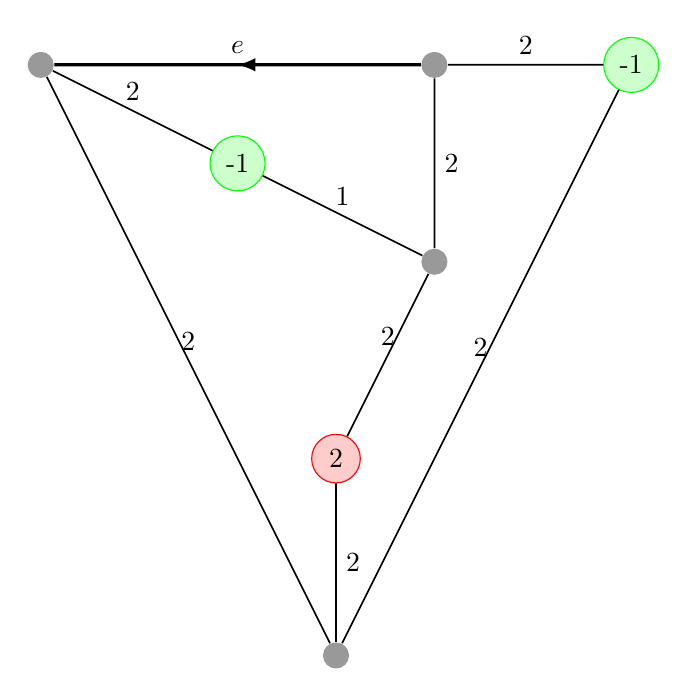
\begin{tikzpicture}
%picture to show how bad path flow augmentation can block arcs such that no simple path can obtain optimality anymore
\node (a) at (0,3)[vertex]{};
\node (s1) at (1,2.5)[source]{-1};
\node (b) at (2,3)[vertex]{};
\node (d) at (2,2)[vertex]{};
\node (c) at (1.5,0)[vertex]{};
\node (s2) at (3,3)[source]{-1};
\node (t) at (1.5,1)[sink]{2};
% \draw[arcflow] (s)--(3)--(t);
\draw[fatarc] (b)--(a)node[pos=0.5, above]{$e$};
% \draw[edge] (a)--(s1)--(d)--(b)--(s2)--(c)--(a);
% \draw[edge] (c)--(t)--(d);
\draw[edge] (a)--(s1)node [pos=0.5, above] {2};
\draw[edge] (s1)--(d)node [pos=0.5, above] {1};
\draw[edge] (d)--(b)node [pos=0.5, right] {2};
\draw[edge] (b)--(s2)node [pos=0.5, above] {2};
\draw[edge] (s2)--(c)node [pos=0.5, above] {2};
\draw[edge] (c)--(a)node [pos=0.5, above] {2};
% \draw[edge] (a)--()node [pos=0.5, above, blue] {2};
\draw[edge] (c)--(t)node [pos=0.5,right] {2};
\draw[edge] (t)--(d)node [pos=0.5, above] {2};
\end{tikzpicture}
\caption{Example graph with capacities on all arcs and demand values at sources and sinks}
 \label{bild:blockingPathflowNet}
\end{figure}

\begin{figure}[h!]
\centering
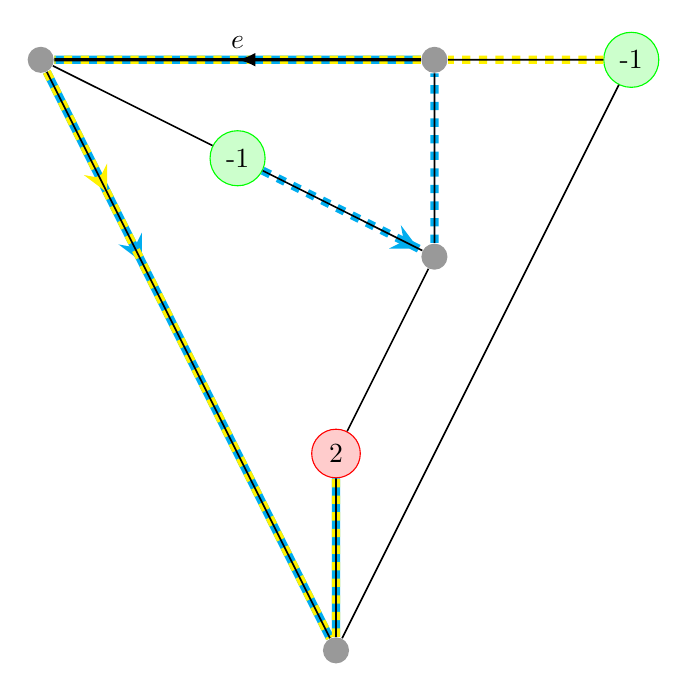
\begin{tikzpicture}
%picture to show how bad path flow augmentation can block arcs such that no simple path can obtain optimality anymore
\node (a) at (0,3)[vertex]{};
\node (s1) at (1,2.5)[source]{-1};
\node (b) at (2,3)[vertex]{};
\node (d) at (2,2)[vertex]{};
\node (c) at (1.5,0)[vertex]{};
\node (s2) at (3,3)[source]{-1};
\node (t) at (1.5,1)[sink]{2};
\draw[arcflow, cyan, dashed] (s1)--(d)--(b);
\draw[arcflow, cyan](b)--(a)--(c)--(t);
\draw[arcflow, yellow, dashed] (s2)--(b)--(a)--(c)--(t);
\draw[fatarc] (b)--(a)node[pos=0.5, above]{$e$};
\draw[edge] (a)--(s1){};
\draw[edge] (s1)--(d){};
\draw[edge] (d)--(b){};
\draw[edge] (b)--(s2){};
\draw[edge] (s2)--(c){};
\draw[edge] (c)--(a){};
\draw[edge] (c)--(t){};
\draw[edge] (t)--(d){};
\end{tikzpicture}
\caption{The optimum - the whole amount of flow is going over $e$ while the flow is still acyclic in the whole network}
 \label{bild:blockingPathflowOpt}
\end{figure}

\begin{figure}[h!]
\centering
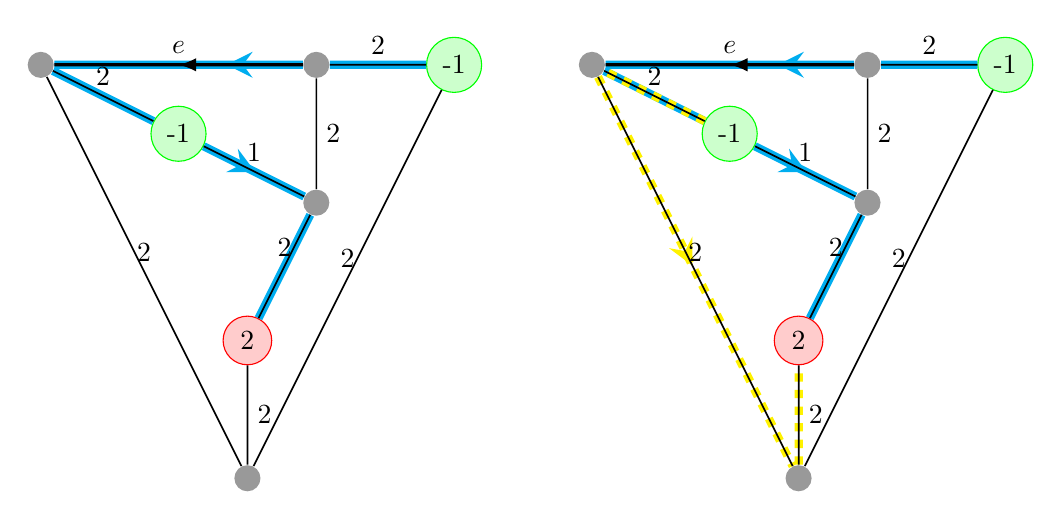
\begin{tikzpicture}
[scale=0.7]
%picture to show how bad path flow augmentation can block arcs such that no simple path can obtain optimality anymore
\node (a) at (0,3)[vertex]{};
\node (s1) at (1,2.5)[source]{-1};
\node (b) at (2,3)[vertex]{};
\node (d) at (2,2)[vertex]{};
\node (c) at (1.5,0)[vertex]{};
\node (s2) at (3,3)[source]{-1};
\node (t) at (1.5,1)[sink]{2};
\draw[arcflow, cyan] (s2)--(b)--(a);
\draw[arcflow, cyan](a)--(s1)--(d)--(t);
% \draw[arcflow, yellow, dashed] (s1)--(a)--(c)--(t);
\draw[fatarc] (b)--(a)node[pos=0.5, above]{$e$};
\draw[edge] (a)--(s1)node [pos=0.5, above] {2};
\draw[edge] (s1)--(d)node [pos=0.5, above] {1};
\draw[edge] (d)--(b)node [pos=0.5, right] {2};
\draw[edge] (b)--(s2)node [pos=0.5, above] {2};
\draw[edge] (s2)--(c)node [pos=0.5, above] {2};
\draw[edge] (c)--(a)node [pos=0.5, above] {2};
\draw[edge] (c)--(t)node [pos=0.5,right] {2};
\draw[edge] (t)--(d)node [pos=0.5, above] {2};
% \draw[edge] (a)--(s1){};
% \draw[edge] (s1)--(d){};
% \draw[edge] (d)--(b){};
% \draw[edge] (b)--(s2){};
% \draw[edge] (s2)--(c){};
% \draw[edge] (c)--(a){};
% \draw[edge] (c)--(t){};
% \draw[edge] (t)--(d){};
\node (2a) at (4,3)[vertex]{};
\node (2s1) at (5,2.5)[source]{-1};
\node (2b) at (6,3)[vertex]{};
\node (2d) at (6,2)[vertex]{};
\node (2c) at (5.5,0)[vertex]{};
\node (2s2) at (7,3)[source]{-1};
\node (2t) at (5.5,1)[sink]{2};
\draw[arcflow, cyan] (2s2)--(2b)--(2a);
\draw[arcflow, cyan](2a)--(2s1)--(2d)--(2t);
\draw[arcflow, yellow, dashed] (2s1)--(2a)--(2c)--(2t);
\draw[fatarc] (2b)--(2a)node[pos=0.5, above]{$e$};
\draw[edge] (2a)--(2s1)node [pos=0.5, above] {2};
\draw[edge] (2s1)--(2d)node [pos=0.5, above] {1};
\draw[edge] (2d)--(2b)node [pos=0.5, right] {2};
\draw[edge] (2b)--(2s2)node [pos=0.5, above] {2};
\draw[edge] (2s2)--(2c)node [pos=0.5, above] {2};
\draw[edge] (2c)--(2a)node [pos=0.5, above] {2};
\draw[edge] (2c)--(2t)node [pos=0.5,right] {2};
\draw[edge] (2t)--(2d)node [pos=0.5, above] {2};
\end{tikzpicture}
\caption{With the given capacities and the already augmented blue flow (left picture) there exists no simple path from 
the middle source to the sink such that 
flow on $e$ could be increased. The best possibility is to augment the dashed yellow path which yields a flow 
value $f(e)=1$ on the maximized arc. This is not optimal as figure \ref{bild:blockingPathflowOpt} showed}
 \label{bild:blockingPathflow}
\end{figure}

This example clearly shows the problems of a path based augmentation approach. A flow could block the wrong arcs while 
the next augmentation step possibly needs these arcs. 
We must give up the idea of finding simple paths and relax them to edge progressions. An edge progression can 
contain arcs and vertices more than once. Thus it can do some kind of cyclic shifting on the flow. Since two flows with 
the same balances in the same network only differ by cyclic flow we can change the flow network to the state we desire. 
Whenever needed the optimal edge progression can do a cyclic shift and afterwards augment the actual path. \\

Here we will not try to deal with the problem of finding such an edge progression. It is likely to be as 
difficult as the acyclic flowbound problem itself. Nevertheless  we describe the algorithm 
in pseudocode (\ref{algo:pathHeur}) to show how such an algorithm would look like if we 
could find such paths or edge progressions and to use it as basis for a heuristic approach.

% 
% Instead we assume we had a blackbox algorithm giving us 
% a path to augment - if necessary augmenting flow back (and by this changing other paths from former iterations) - such 
% that the result is an acyclic flow and uses a specified arc if required. We show how such an algorithm could be used to 
% compute an upper bound for the flow on the specified arc of a network.\\
% 
% %algo um mit dieser blackbox die optimale flussschranke zu berechnen!
% 
% We will specify the heuristic algorithm here in pseudocode and show that it yields a valid bound not higher than the 
% sum of flow from all sources. %We will also analyze its worst-case running time.TODO?

%Pseudocode des Algorithmus
\begin{algorithm}
 \caption{path based heuristic flow bound algorithm}
\label{algo:pathHeur}
 %TODO gehe gerade von vorwärts gerichteter e aus, und maximierung
 \begin{algorithmic}[5]%[0] means no line numbers, n means every nth line number is displayed
  \Function{Heuristic}{$G=(V,A),\, e=(u,v)\in A,\, b:V\to \R $}%hier übergabeparameter
    \State define $b':V\to \R,\, b'(v)\gets 0 \forall v\in V$ \Comment{temporary balances}
    \State define $f: A\to\R,\, f(v)\gets 0 \forall a\in A$
    \While {$\neg (b+b'\equiv 0) $}\Comment{while there are active source-sink-pairs}
      \If{ $c(e)>f(e)$}
      \State choose active source $v\in V$ 
	\State $P\gets $\Call{acyclicEdgeProgOverE}{$v, e$}
	  %\Comment{find augmentable path over $e$ such that we still have acyclic flow after augmentation}
	\If{$P\ne \emptyset $}
	  \State \Call {maxAugment}{$P$}\label{heur:lineAugCase1}
	  \State \textbf{continue}
	\EndIf
      \EndIf
%       \Else
	\State choose $s\in V$ with $b(s)+b'(s)<0$\Comment{source that is still active}
	\State $c_{alt}(e)\gets c(e)$\Comment{save old capacity value}
	\State $c(e)\gets f(e)$\Comment{make $e$ blocked for a short time}
	\State $P\gets$\Call{acyclicEdgeProg}{$s$}\Comment{try finding a path that avoids $e$}
	\State $c(e)\gets c_{alt}(e)$
	\If{$P\ne \emptyset$}
	  \State \Call {maxAugment}{$P$}\label{heur:lineAugCase2}
	  \State \textbf{continue}
	\Else
	  \State $P\gets$ \Call{acyclicEdgeProg}{$s$}
		\Comment{try to find any augmentable path, at this point of time it will be decreasing the flow on $e$}
	  \If{$P\ne \emptyset$}
	    \State \Call {maxAugment}{$P$}\label{heur:lineAugCase3}
	    \State \textbf{continue}
	  \Else
	    \State \Return problem infeasible
	  \EndIf
	\EndIf
    \EndWhile
    \State \Return $f(e)$
  \EndFunction
%   \algstore{heur}
 \end{algorithmic}

\end{algorithm}

%algo um maximum zu augmentieren
\begin{algorithm}
 \begin{algorithmic}
  \Function {maxAugment}{$P$}
    \State $s \gets $ source node of $P$
    \State $t \gets $ sink node of $P$
    \State augval $\gets \min(|s|,|t|)$
    \ForAll{$a\in P$}
      \State arcMaxAugval $\gets$ max augmentable flow in direction of $P$ on $a$ 
      \State augval $\gets \min($augval, arcMaxAugval)
    \EndFor
    \ForAll{$a\in P$}
%       \If{$a$ is considered the second time in the same direction in $P$}
% 	\State \textbf{continue}\Comment do not increase flow value here, equivalent to increase of capacity bounds on 
% 		this arc. Why this is necessary see example \ref{example:mustNotAugmentArcTwice}
%       \EndIf
      \State increase flow on $a$ in direction of $P$ by augval
    \EndFor
    \State $b'(s) \gets b'(s) + $augval
    \State $b'(t) \gets b'(t) - $augval
  \EndFunction
 \end{algorithmic}
\end{algorithm}

\begin{prop}
 The described algorithm \ref{algo:pathHeur} together with a function \textit{acyclicEdgeProg()} 
 resp. \textit{acyclicEdgeProgOverE} 
 that finds an augmentable edge progression (acyclicEdgeProgOverE using a specified arc $e$)
 whose augmentation is not causing any flow cycles computes the optimal bounds to the acyclic flowbound problem. 
\end{prop}
\begin{proof}
 We assume that the blackbox algorithm for finding an acyclic edge progression is correct. An edge progression can use
 arcs more than once $\Rightarrow$ it can do cyclic shifting on every cycle in the same connected component: 
 For every cyclic shift that is necessary it chooses an augmentable path towards the cycle, then goes around the cycle 
 and on the same way back. If there is no augmentable path unto a cycle in the same connected component there has to be
 a directed cut that is at its capacity bounds. But in this case this cycle (and everything behind the cut) cannot 
 influence the acyclic path at all.
 If the algorithm can change the flow on every cycle, it can produce every acyclic flow that is possible (before augmenting).
 There is always a path if there is any acyclic flow with this flow value on $e$ because every acyclic flow can be 
 decomposed into flow on simple paths. So the optimal edge progression could detect the right $s-t$-path, produce the 
 acyclic flow without this path and then augment. So if the algorithm does not find any edge progression, there 
 is also no acyclic flow with a higher flow value on $e$.  
\end{proof}

So we have seen that augmentation algorithms could only work with a too powerful algorithm that shifts flow before 
augmenting on a path. The main problem is that a flow can unnecessarily block an arc that is needed in a later stage 
of the algorithm. 

So the following idea for a heuristic algorithm comes in: Can we increase the capacity bounds of the arcs in a way 
such that they can only be blocked in the case when the acyclic flow bound is reached?\\

Yes: if we double the capacities there will be no more flows blocked if not necessary: Even in flows that do not 
require acyclicity an upper bound for flow on an arc $e$ is the flow that can be sent from sources to one end of the 
maximized arc $e$ as well as the flow that can be sent from the other end of $e$ to sinks. This flow can be computed by 
the standard maximum flow algorithms where path augmentation works well. But on each part of the problem - maximum flow 
from sources to one end of $e$ and maximum flow from the other end vertex of $e$ to sinks - the capacity of each arc in 
the network can only be used one time. So combining these two would give twice the capacity at most. Thus we can 
conclude that a more restricted problem (like finding the acyclic bound) can not need more capacity than this on a 
single arc.\\

We will describe an equivalent variant of this idea in the next section more detailed.
 

\newpage
\subsection{A Simple Heuristic Approach}

As we have seen, the computations of the MIP formulation with separation of the Acyclicity Constraints could be 
expensive in running time and ressource consumption. The solved problem is a relaxation of the real-world 
problem anyway, so we can as well think 
about different relaxations and heuristic approaches. This chapter will introduce a simple and easy to 
implement heuristic approach inspired by the idea of the former section, where we showed why path augmentation models 
do not work for the acyclic flowbound problem. This approach uses a graph transformation and computes a Minimum Cost 
Flow on the transformed graph. We show that we get a valid bound for the Acyclic Flowbound Problem from this 
transformed graph.\\

The main idea of this heuristic approach is to avoid that the same flow is cycling over and over again until it reaches 
the capacity bounds. The path augmentation of the section before could achieve this goal. But we need to relax the 
capacity bounds and by this we relax also the problem. The proof that it suffices to double the capacities relies on 
the idea of distinguishing the flow before and after the maximized arc, because in every part of this the capacities 
have to be respected. If we double capacities and compute flow in this network it could happen that flow in one part 
uses 1.5 times of an arcs capacity and the other only half of it. So the bounds get in fact tighter if we separate the 
two parts.

In order to achieve this we make two copies of the original graph and make the arc we maximize the 
bridge between the two. On one part of the graph we only have sources, on the other part we only have sinks. 
In order to make the problem feasible we introduce artificial arcs between the sinks and their counterparts in the other 
copy of the graph. These artificial arcs get a detention cost so they are only used when there is no other way. On this 
modified graph we obtain minimum costs by sending as much flow as possible over the maximized arc. We can add the flow 
in both parts in the end, obtaining a flow for the original graph that might be not acyclic and not respecting the 
capacities but has maximum flow value on the arc we maximize. 

Let us describe the approach in a formal way.

\subsubsection*{The Graph Transformation}

The following algorithm \ref{algo:graphtransform} describes how the graph is transformed to the new graph. It mainly 
splits the graph into two copies $X$ and $Y$, sets costs and introduces links between both parts and the 
supersource and supersink.

%Pseudocode des Algorithmus
\begin{algorithm}
 \caption{graph transformation}
 \label{algo:graphtransform}
 \begin{algorithmic}[5]
  \Function{MakeTransformedGraph}{$G=(V,A), e\in A$}
  \State create empty graph $G':=(V',A'), V'=A'=\emptyset$
  \State create labels capacity $A'\to \R$, cost $A'\to \R$% , demand $V'\to\R$
  \State create $s, t\in V$ \Comment{ supersource and supersink}
  \State create $a_0 :=(s,t) \in A'$
  \State capacity$(a_0)\gets\infty$ 
  \State cost$(a_0)\gets 2$ \Comment{highest arc cost in the network}
  \ForAll{$v\in V$}\Comment{make two copies of each node}
    \State create $v_X, v_Y\in V'$
    \If{$v$ is source of $G$}
      \State create arc $a:=(s,v_X)\in A'$
      \State capacity$(a)\gets$ supply$(v)$
    \ElsIf{$v$ is sink of $G$}
      \State create arc $a:=(v_X, t)\in A'$
      \State create arc $b:=(v_Y,t)\in A'$
      \State cost$(a)\gets 1$
    \EndIf
  \EndFor
  \ForAll{$a=(u,v)\in A$}
    \If{$a=e$}\Comment{for the arc to maximize we only make a bridge, no copy}
      \State create arc $e':=(u_X, v_Y)\in A'$
      \State capacity$(e')\gets$ capacity$(e)$
    \Else
      \State create arcs $a_X:=(u_X, v_X), a_Y:=(u_Y, v_Y)\in A'$
      \State capacity$(a_X)\gets$ capacity$(a)$, capacity$(a_Y)\gets$ capacity$(a)$
      \State cost$(a_X)\gets 0$, cost$(a_Y)\gets0$
    \EndIf
  \EndFor
  \State \Return $G'$
  \EndFunction
 \end{algorithmic}

\end{algorithm}

Figure \ref{bild:graphtransform} shows as an example how the graph from the last section would be transformed by this 
algorithm

\begin{figure}[h!]
\centering
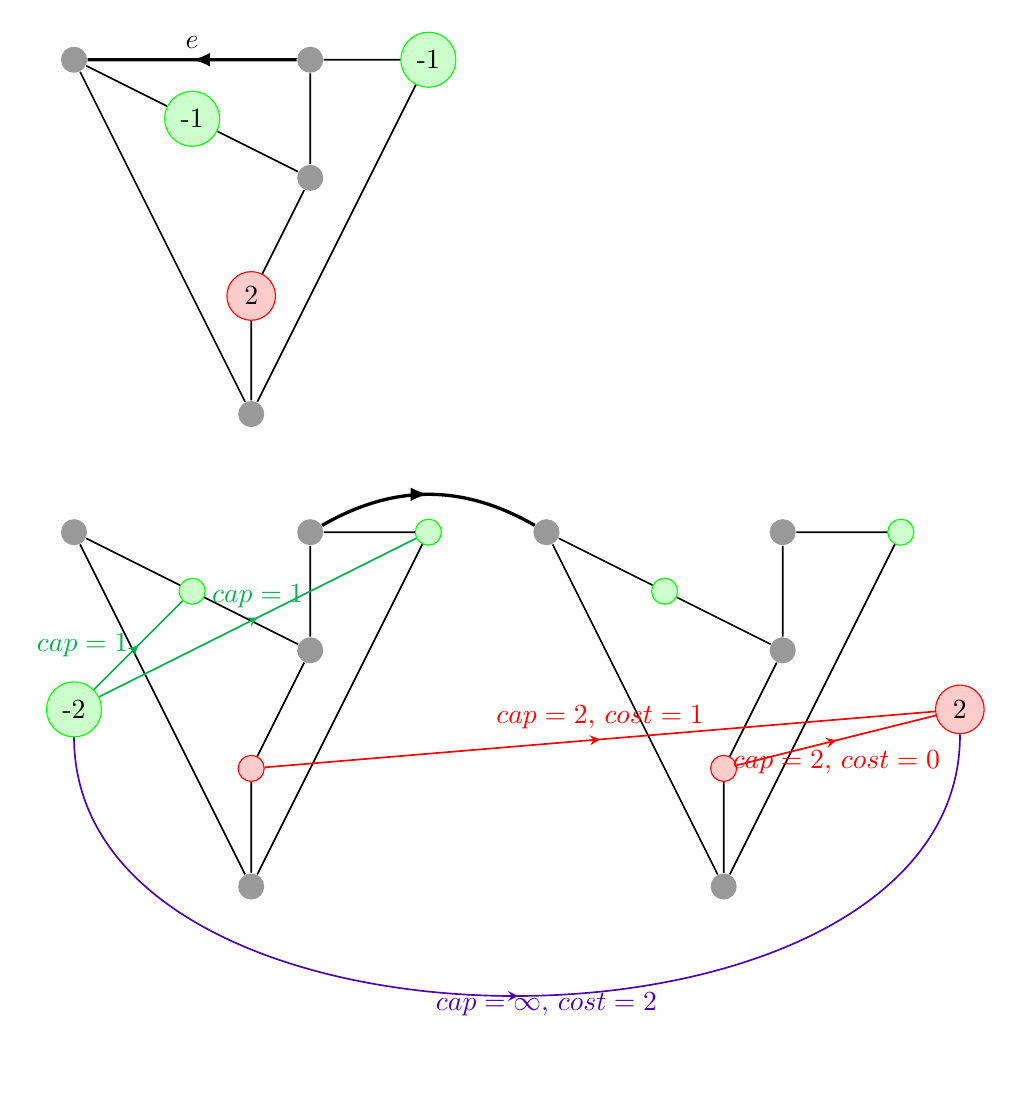
\begin{tikzpicture}[scale=0.6]
\node (a) at (0,3)[vertex]{};
\node (s1) at (1,2.5)[source]{-1};
\node (b) at (2,3)[vertex]{};
\node (d) at (2,2)[vertex]{};
\node (c) at (1.5,0)[vertex]{};
\node (s2) at (3,3)[source]{-1};
\node (t) at (1.5,1)[sink]{2};
% \draw[arcflow, cyan, dashed] (s1)--(d)--(b);
% \draw[arcflow, cyan](b)--(a)--(c)--(t);
% \draw[arcflow, yellow, dashed] (s2)--(b)--(a)--(c)--(t);
\draw[fatarc] (b)--(a)node[pos=0.5, above]{$e$};
\draw[edge] (a)--(s1){};
\draw[edge] (s1)--(d){};
\draw[edge] (d)--(b){};
\draw[edge] (b)--(s2){};
\draw[edge] (s2)--(c){};
\draw[edge] (c)--(a){};
\draw[edge] (c)--(t){};
\draw[edge] (t)--(d){};

%supersource und supersink
\node(sups) at (0,-2.5)[source]{-2};
\node(supt) at (7.5,-2.5)[sink]{2};

\node (la) at (0,-1)[vertex]{};
\node (ls1) at (1,-1.5)[source]{};
\node (lb) at (2,-1)[vertex]{};
\node (ld) at (2,-2)[vertex]{};
\node (lc) at (1.5,-4)[vertex]{};
\node (ls2) at (3,-1)[source]{};
\node (lt) at (1.5,-3)[sink]{};
% \draw[fatarc] (lb)--(la)node[pos=0.5, above]{$e$};
\draw[edge] (la)--(ls1){};
\draw[edge] (ls1)--(ld){};
\draw[edge] (ld)--(lb){};
\draw[edge] (lb)--(ls2){};
\draw[edge] (ls2)--(lc){};
\draw[edge] (lc)--(la){};
\draw[edge] (lc)--(lt){};
\draw[edge] (lt)--(ld){};

\node (ra) at (4,-1)[vertex]{};
\node (rs1) at (5,-1.5)[source]{};
\node (rb) at (6,-1)[vertex]{};
\node (rd) at (6,-2)[vertex]{};
\node (rc) at (5.5,-4)[vertex]{};
\node (rs2) at (7,-1)[source]{};
\node (rt) at (5.5,-3)[sink]{};
\draw[fatarc, bend left] (lb)to(ra);
\draw[edge] (ra)--(rs1){};
\draw[edge] (rs1)--(rd){};
\draw[edge] (rd)--(rb){};
\draw[edge] (rb)--(rs2){};
\draw[edge] (rs2)--(rc){};
\draw[edge] (rc)--(ra){};
\draw[edge] (rc)--(rt){};
\draw[edge] (rt)--(rd){};
\draw[arc, green!70!blue] (sups)--(ls1)node[pos=0.5, left]{$cap=1$};
\draw[arc, green!70!blue] (sups)--(ls2)node[pos=0.5, above]{$cap=1$};
\draw[arc, red] (rt)--(supt)node[pos=0.5, below]{$cap=2,\, cost=0$};
\draw[arc, red] (lt)--(supt)node[pos=0.5, above]{$cap=2,\, cost=1$};
\draw[arc, purple!40!blue, bend right =90] (sups)to(supt)node at (4,-5){$cap=\infty,\,cost=2$};

\end{tikzpicture}
\caption{The transformation of the example network from the former section}
 \label{bild:graphtransform}
\end{figure}


With this transformation and any algorithm for Minimum Cost Flow we can set up an algorithm for our problem. 
For the Maximum Flow and Minimum Cost Flow Problem in graphs there are many standard algorithms we could use. The 
classical Maximum Flow algorithm of Ford and Fulkerson \cite{Ford-Fulkerson_algo} arising from their Max-Flow-Min-Cut 
theorem is based on augmenting flow on source-sink-paths in the network as well as the improved algorithms of Edmonds 
and Karp \cite{EdmondsKarp1972} or Dinic \cite{Dinic1970}. Algorithms for Maximum Flow can be used to first check if 
there is any feasible flow in the network. If there is no feasible flow we can give up at this point, while the flow 
problem on the transformed graph is always feasible by construction.

Deriving from the Max-Flow Algorithms there are many algorithms solving the Min-Cost-Flow Problem. Edmonds and 
Karp described a Successive Shortest Path Algorithm in \cite{EdmondsKarp1972}. Goldberg and Tarjan proposed the Minimum 
Mean Cycle Cancelling Algorithm \cite{minMeanCycleCancelling89} with runnning time of $\mathcal{O}(nm(log 
n)\min\{log(nC), m log n\}) $. %TODO fuer die anderen ebenfalls laufzeiten odr fuer keine
Another algorithm is the Network Simplex by Orlin \cite{NetworkSimplexOrlin97} (which was used in the computational 
study) There are a lot more algorithms available for Minimum Cost Flow.

Our algorithm mainly consists of a feasibility test, a transformation of the graph $G$ and a Minimum Cost Flow 
computation on the transformed graph $G'$, see algorithm \ref{algo:simpleheur}. 

\begin{algorithm}
 \caption{simple heuristic}
 \label{algo:simpleheur}
 \begin{algorithmic}
  \Function{FlowBoundHeur}{$G=(V,A), e\in A$}
  \State mf$\gets$ \Call{MaxFlow}{G}
  \If{mf < nominated ingoing flow}
    \State\Return infeasible
  \EndIf
  \State $G'=$ \Call{MakeTransformedGraph}{$G,e$}
  \State $f\gets$ \Call{MinCostFlow}{$G'$}
  \State ub$\gets f(e')$
  \State backwardflow$\gets f(a_0)$
  \State \Return ub - backwardflow
  \EndFunction
 \end{algorithmic}
\end{algorithm}

We show the correctness of the algorithm: %TODO and running time? dependent on used mincostflow!

\begin{figure}[h!]
\centering
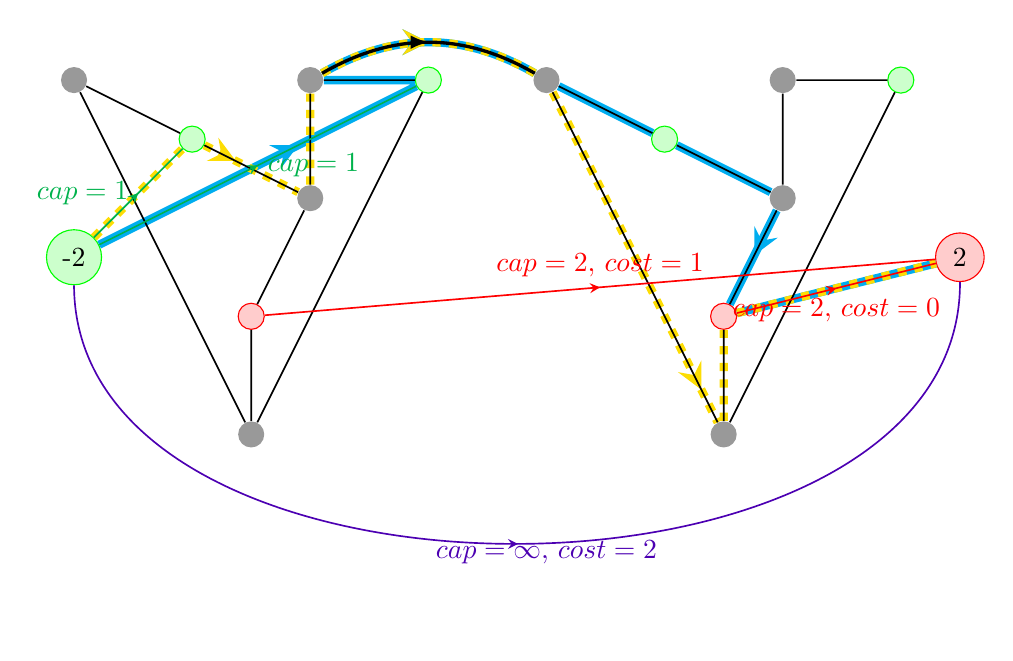
\begin{tikzpicture}[scale=0.6]
%supersource und supersink
\node(sups) at (0,-2.5)[source]{-2};
\node(supt) at (7.5,-2.5)[sink]{2};
%left part
\node (la) at (0,-1)[vertex]{};
\node (ls1) at (1,-1.5)[source]{};
\node (lb) at (2,-1)[vertex]{};
\node (ld) at (2,-2)[vertex]{};
\node (lc) at (1.5,-4)[vertex]{};
\node (ls2) at (3,-1)[source]{};
\node (lt) at (1.5,-3)[sink]{};
%right part
\node (ra) at (4,-1)[vertex]{};
\node (rs1) at (5,-1.5)[source]{};
\node (rb) at (6,-1)[vertex]{};
\node (rd) at (6,-2)[vertex]{};
\node (rc) at (5.5,-4)[vertex]{};
\node (rs2) at (7,-1)[source]{};
\node (rt) at (5.5,-3)[sink]{};

\draw[arcflow, cyan] (sups)--(ls2)--(lb);
\draw[arcflow, cyan, bend left] (lb)to (ra);
\draw[arcflow, cyan](ra)--(rs1)--(rd)--(rt)--(supt);
\draw[arcflow, yellow!80!orange, dashed](sups)--(ls1)--(ld)--(lb);
\draw[arcflow, yellow!80!orange, dashed, bend left](lb)to(ra);
\draw[arcflow, yellow!80!orange, dashed](ra)--(rc)--(rt)--(supt);

\draw[edge] (la)--(ls1){};
\draw[edge] (ls1)--(ld){};
\draw[edge] (ld)--(lb){};
\draw[edge] (lb)--(ls2){};
\draw[edge] (ls2)--(lc){};
\draw[edge] (lc)--(la){};
\draw[edge] (lc)--(lt){};
\draw[edge] (lt)--(ld){};
\draw[fatarc, bend left] (lb)to(ra);
\draw[edge] (ra)--(rs1){};
\draw[edge] (rs1)--(rd){};
\draw[edge] (rd)--(rb){};
\draw[edge] (rb)--(rs2){};
\draw[edge] (rs2)--(rc){};
\draw[edge] (rc)--(ra){};
\draw[edge] (rc)--(rt){};
\draw[edge] (rt)--(rd){};
\draw[arc, green!70!blue] (sups)--(ls1)node[pos=0.5, left]{$cap=1$};
\draw[arc, green!70!blue] (sups)--(ls2)node[pos=0.5, right]{$cap=1$};
\draw[arc, red] (rt)--(supt)node[pos=0.5, below]{$cap=2,\, cost=0$};
\draw[arc, red] (lt)--(supt)node[pos=0.5, above]{$cap=2,\, cost=1$};
\draw[arc, purple!40!blue, bend right =90] (sups)to(supt)node at (4,-5){$cap=\infty,\,cost=2$};
\end{tikzpicture}
\caption{This flow has zero costs, is feasible in the heuristic and has the optimum value $f(e)=2$}
 \label{bild:graphtransformWithFlow}
\end{figure}

\begin{prop}
 The heuristic algorithm \ref{algo:simpleheur} returns a valid upper bound for the possible acyclic flow on a given 
 arc $e$ in the network, or infeasible if there is no feasible network flow for the given flow balances at sources and 
 sinks.
\end{prop}

\begin{proof}
\textbf{Feasibility Test: }We have to show that the ordinary feasibility test with maximum flow is sufficient even for 
acyclic flow: If the flow network nomination (in- and outflow) is infeasible, no algorithm for the 
maximum flow problem will find a flow that is fulfilling these balances completely. Then also for the stricter acyclic 
flow problem this is infeasible. The other direction is also true: if there is a feasible flow, there also is a 
feasible acyclic flow:

Take the maximum flow and choose one flow cycle within (If there is none we are done). On all arcs of the cycle the 
flow is going in the same direction in relation to the cycle. We can choose the minimum flow on the cycles arcs and 
reduce flow on each arc of the cycle by this amount. The resulting flow is still a feasible flow, but we removed the 
flow cycle. This can be done until the flow is acyclic. But if there is any acyclic flow, there also has to be an 
acyclic flow that is maximum on the arc we are interested in. So in order to test feasibility it is enough to run a 
ordinary maximum flow algorithm.\\


\textbf{Relaxation: }To prove that we get an upper bound with this heuristic we have to show that the result we 
get is the maximum value of a relaxation of the problem. 

If a flow is acyclic we can decompose it into flow on a set of simple paths. This means that 
the Acyclic Flowbound Problem could theoretically be solved by an algorithm augmenting simple paths (in the 
right order) where we put some extra constraints and objectives on these paths. These extra constraints have to forbid 
the closing of any flow cycle by the path as well as forcing the path to use arc $e$ if possible. (Section 
\ref{model:pathaugment} describes this idea and shows the difficulties of choosing the right path for augmentation.)
%TODO koennte das modell einzeln hinschreiben mit 
%hinweis auf NP schwere von constrained shortest path. anschließend kommt das relaxierungsargument besser !!!
%Außerdem hätte ich damit shconmal ein gutes modell

The heuristic algorithm is a relaxation of this constrained path augmentation model. It still forces all paths to go 
over $e$ if possible (which might be much more since it is a problem with weaker conditions). 
We can reconstruct a flow in the original graph from the flow in the transformed graph by summing up the flow values on 
both copied arcs, assigning this flow to the original arc: $f(a)=f'(a_X)+f'(a_Y)$ and the assigned flow value of the 
bridge arc to the maximized arc of the original problem. 

All the flow conservation constraints still hold after constructing the flow in the original graph from the two copies:
\begin{align*}
& \sum_{a\in \delta^+(v)}q_a - \sum_{a\in\delta^- (v)}q_a &=& d_v\ &\forall v\in V_X \\
+& \sum_{a\in \delta^+(v)}q_a - \sum_{a\in\delta^- (v)}q_a &=& d_v\ &\forall v\in V_Y \\
=& \sum_{a\in \delta^+(v_X)\cup\delta^+(v_Y)}q_a - \sum_{a\in\delta^- (v_X)\cup\delta^-(v_Y)}q_a &=& d_v\ &\forall 
v_X\in V_X, v_Y\in V_Y \\
=& \sum_{a\in \delta^+(v)}q_a - \sum_{a\in\delta^- (v)}q_a &=& d_v\ &\forall v\in V \\
\end{align*}

The flow balances at sources and sinks are set right by construction.\\

When no more flow can be sent over the maximized arc $e$ the path augmentation model already gives a valid bound 
if the flow is feasible. But in fact this model can determine the amount of flow that is necessary to augment backwards 
on $e$ in a path model.

We distinguish whether the flow is going over the bridge $e$, going to a sink node in already in part $X$ of the 
transformed graph and thus having costs of 1 per unit, 
or is going from $s$ to $t$ directly with a cost of 2 per unit. The flow with costs of 2 cannot be sent over $e$ in 
forward direction neither find any sink in part $X$ of the graph. If there is a feasible flow in $G$ (which we tested) 
the only possible way is that the remaining flow has to go backward over $e$. So we can reduce the flow on the 
bridge by this amount of flow directly going from $s$ to $t$ and the bound is still valid. (In algorithm 
\ref{algo:pathHeur} from the section before this would be the part in line \ref{heur:lineAugCase3} where flow is 
augmented backwards).\\

$\Rightarrow$ Since the problem is just a relaxation of the original problem/the constrained simple path model, the 
obtained bound is always weaker (in this case $\ge$) than the optimal bound for maximum acyclic flow. 
$\Rightarrow$ the heuristic is correct for finding upper bounds for the acyclic flow on an arc.

\end{proof}%TODO der beweis ist lang und unuebersichtlich, man koennte fragen wozu man manche erklaerungen braucht.

So we have seen that we can compute an upper bound via the optimum for this relaxed problem with a fast standard 
algorithm for maximum flows that can be retranslated into the original problem. 
However, the capacity constraints of the original problem might be violated after retranslation. We set the arcs 
capacities in part $X$ and part $Y$ both to the value of the original capacities. Thus it might happen that actual flow 
value in the original graph sums up to a higher value than the capacity allows (up to twice the capacity). 


\begin{figure}[h!]
\centering
\begin{tikzpicture}
\node (a) at (0,-6)[vertex]{};
\node (s1) at (1,-6.5)[source]{-1};
\node (b) at (2,-6)[vertex]{};
\node (d) at (2,-7)[vertex]{};
\node (c) at (1.5,-9)[vertex]{};
\node (s2) at (3,-6)[source]{-1};
\node (t) at (1.5,-8)[sink]{2};
% \draw[arcflow, cyan, dashed] (s1)--(d)--(b);
\draw[arcflow, cyan](s2)--(b);
\draw[arcflow, cyan](b)--(a)--(s1)--(d);
\draw[arcflow, cyan](d)--(t);
\draw[arcflow, yellow!70!orange, dashed] (s1)--(d);
\draw[arcflow, yellow!70!orange, dashed] (d)--(b)--(a)--(c);
\draw[arcflow, yellow!70!orange, dashed] (c)--(t);
\draw[fatarc] (b)--(a)node[pos=0.5, above]{$e$};
\draw[edge] (a)--(s1){};
\draw[edge] (s1)--(d)node(errpos)[pos=0.5]{};
\draw[edge] (d)--(b){};
\draw[edge] (b)--(s2){};
\draw[edge] (s2)--(c){};
\draw[edge] (c)--(a){};
\draw[edge] (c)--(t){};
\draw[edge] (t)--(d){};
\node (err) at (-1,-7)[ellipse, red, draw=red]{ $f(a)=2>cap(a)=1$};
\draw[->, stealth, semithick, bend right,red](err)to(errpos);
\draw[ultra thick, ->, red!50] (1.55,-6.2) arc (30:330:0.2);
% \draw[pattern=dots, pattern color=red](a)--(s1)--(b);%(0,-6)--(1,-6)--(1,-5);
%TODO man könnte doch kreisfluss umschlossenes gebiet rot füllen?
\end{tikzpicture}
\caption{If we retransform the flow from figure \ref{bild:graphtransformWithFlow} (which is feasible in the heuristic) 
to the original network we get a violated capacity constraint on the arc with $c=1$. The flow is not acyclic anymore 
either.}
 \label{bild:graphretransformWithFlow}
\end{figure}
Also we cannot guarantee the acyclicity anymore. It might happen that we have cyclic flow in our 
original graph $G$ even if the flow in the transformed graph $G'$ was acyclic. This happens when paths from 
the different parts $X$ and $Y$ of $G'$ are crossing after they are brought back to the original graph $G$ to 
build a solution there. For an example see figure \ref{bild:graphretransformWithFlow} which is the retransformation of 
the example flow in figure \ref{bild:graphtransformWithFlow}.

\newpage
\section{Implementation and Computational Results}% The models we described have also been implemented and tested on networks of different size.
In this section we will discuss practical implementation and results of the computation. For relevant real-world 
problem sizes the exact algorithm (even with separation of the acyclicity constraints) is too slow. Hence we also 
describe how to relax the problem in order to get useable (though in general not optimal) results for the flow bounds. 
We compare the bounds found by different approaches/settings in different networks and nominations to see which 
approach is suited best to actually compute acyclic flow bounds in a network. 

At last we compare the impact of bounds and the number of fixed variables fed into the solver on the model sizes of the 
discretization. \\

\subsection{Implemented and Tested Algorithms}

We described the theoretical backgrounds of different algorithms to obtain flow bounds for our problem. The 
computational results of different implementations of them may vary widely, and the performance is influenced by lots 
of details regarding the machines, programming languages, data structures or just code quality. Nevertheless we want 
to give an overview what worked well in the implementation and what did not.\\

All algorithms where tested on a PC with instances of the \textit{"gaslib"} gasnet test library. The library can be 
downloaded on \url{http://gaslib.zib.de/}. A detailed description of this problem library can be found in 
\cite{HumpolaJoormannOucherifPfetschScheweSchmidtSchwarz:2015}.

\subsubsection{MIP with Node Potentials and Binary Direction Variables}
The MIP model described in \ref{model:nodePotential} was implemented in Lamatto, using Gurobi as solver for this 
model. However,the two layers of indicator constraints seem to be a heavy problem of the model in 
practice. The folowing model was implemented:
\begin{align*}
  &\min \sum_{a\in A} w_a\cdot q_a & \\
 s.t. & \sum_{a\in \delta^+(v)}q_a - \sum_{a\in\delta^- (v)}q_a &=& d_v\ &\forall v\in V \\
 & q_a &\le& c_u(a) & \forall a\in A\\
 & q_a &\ge& c_l(a) & \forall a\in A\\
 & \rho_{vw}=1 &\Rightarrow &\pi_v\ge\pi_w +1 & \forall (v,w)\in A\\
 & \rho_{vw}=0 &\Rightarrow &\pi_w\ge\pi_v +1& \forall (v,w)\in A\\
 & \rho_{vw}=1 &\Rightarrow &q((v,w))\ge 0& \forall (v,w)\in A\\
 & \rho_{vw}=0 &\Rightarrow &q((v,w))\le 0& \forall (v,w)\in A\\
 & q_a \in \R & & &\forall a\in A\\
 & \pi_v \in \R & & & \forall v\in V\\
 & d_a \in \{0,1\} & & &\forall a\in A\\
 & \rho_{vw} \in \{0,1\}&&& \forall a=(v,w)\in A\\
\end{align*}
Integer node potentials imply the direction of the arc between the incident nodes. These binary direction 
variables again imply the sign of the actual flow on an arc. Indicator constraints are usually implemented via 
Big-M-constraints of the form 
\begin{align*}
 &\pi_v-\pi_w &\ge & N(\rho_{vw}-1)+1\\
 &\pi_v-\pi_w&\le &N\rho_{vw}-1 \\
 &q((v,w))&\ge& M(\rho_{vw}-1)\\
 &q((v,w))&\le & M\rho_{vw}\\
 &\rho_{vw} \in \{0,1\}&&\\
\end{align*}
with sufficient big values for $M$ and $N$. This model heavily relies on the Big-M-constraints.
For any MIP solver these indicator or big-M constraints are difficult to handle, because the optimal vertex of the LP 
polyhedron can be quite far from the optimal mixed integer solution.\\

The model was tested on the smallest network named "gaslib-40" of the gaslib package. After running for 
%TODO testergebnisse (vermutlich fail nach etlichen tagen)

\subsubsection{MIP with Binary Direction Variables and separated Acyclicity Constraints}
In section \ref{model:AcyclicityConstraints} we described a model using acyclicity constraints on the binary directions 
for cycle that was found during the solving process.


\newpage
\section{Summary}




\newpage
\newpage
\addcontentsline{toc}{section}{Bibliography}
\bibliographystyle{amsplain}
% \bibliographystyle{apalike}
\bibliography{literatur}
\nocite{*}

\end{document}
